% 第 10 章 流形与流形上的形式
\chapter{流形与流形上的形式}

本章我们以某种更数学上严格的方式重新引入流形，同时努力不让你被细节淹没. 一如既往，我们仍将把重点放在概念理解和宏观图景上. 流形理论是一个浩瀚而丰富的主题，有许多书以完全严格的方式介绍流形，并把所有繁琐的技术细节都明确写出. 当你理解本章之后，你就准备好去啃这些书了.

第 1 节重新引入流形，而第 2 节重新引入切空间的思想. 第 3 节给出向量\newterm{push-forward}{前推}{push-forward}和形式\newterm{pull-back}{拉回}{pull-back}的抽象表述. 然后我们在第 4 节讨论流形上的微分形式以及微分和积分. 尽管一般流形是比 $\mathbb{R}^n$ 更抽象的背景，但你不应感到意外的是，你已经熟悉的大部分概念性思想都会基本上原封不动地延续过来. 从这种意义上说，我们只是在重复我们已经做过的事情，只不过是在一个更抽象的背景下.

\section{流形的定义}

在本书开头，我们花大力气区分了流形 $\mathbb{R}^n$ 与向量空间 $\mathbb{R}^n$. 流形 $\mathbb{R}^n$ 在每个点 $p$ 处的切空间，即空间 $T_p(\mathbb{R}^n)$，等价于向量空间 $\mathbb{R}^n$. 我们告诉过你，我们做出这一区分是因为一般地，大多数流形根本不是向量空间. 大多数流形缺少欧几里得空间——即我们在整个微积分课程中处理过的那些流形——所具有的许多重要性质. 本节一开始我们就试图更详细地解释这一点.

如你所知，流形是通常可以认为局部为欧几里得的空间；这意味着如果你放大流形的某个点，那个点的非常小的邻域本质上看起来就像某个 $n$ 的流形 $\mathbb{R}^n$，见图~\ref{fig:2-8} 至图~\ref{fig:2-10}. 正因为如此，人们实际上可以像在流形 $\mathbb{R}^n$ 上做微积分那样在流形上做微积分.

然而，流形与欧几里得空间 $\mathbb{R}^n$ 之间有一些明显的差别. 首先，在欧几里得空间 $\mathbb{R}^n$ 中，有一种自然的把切向量\newterm{parallel-transport}{平行移动}{parallel transport}到另一点的方式. 例如，当我们把向量 $\binom{2}{1}_p\in T_p\mathbb{R}^2$ 平移到 $\binom{2}{1}_q\in T_q\mathbb{R}^2$（其中 $p\neq q$）时，这两个向量以直观明显的方式彼此平行. 见图~\ref{fig:10-1}. 事实上，这太明显了，以至于我们很少去想，为了知道两个不同点处的向量是否彼此平行，我们需要做出哪些潜在的、未言明的假设.

\begin{figure}[htbp]
  \centering
  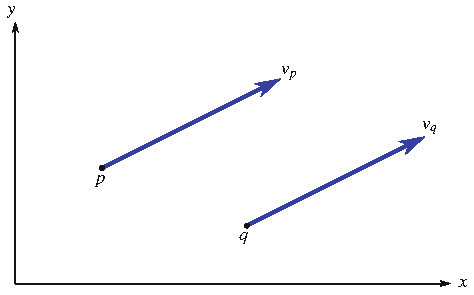
\includegraphics[width=0.562\linewidth]{images/vector/fig-10-1.pdf}
  \caption{向量 $2e_1+e_2$ 画在流形 $\mathbb{R}^2$ 中的两个不同点 $p$ 和 $q$ 处. 这两个向量以直观明显的方式彼此平行}
  \label{fig:10-1}
\end{figure}

正如我们以前讨论过的，$S^2$ 是一个流形，因为 $S^2$ 的每个点的小邻域看起来都像 $\mathbb{R}^2$. 然而，考虑图~\ref{fig:10-2} 所示的 $S^2$，其中点 $p$ 是``北极''，点 $q$ 在``赤道''上. 现在考虑 $v_p\in T_pS^2$. $T_qS^2$ 中什么样的向量可以在某种意义上被认为是与 $v_p$ 平行的？也就是说，把 $v_p$ 平行移动到点 $q$ 的结果是什么？从图~\ref{fig:10-2} 中显然看不出这一点. 事实证明，为了找到流形上向量的平行移动，需要在流形上添加某种附加结构. 这种附加结构称为\newterm{connection}{联络}{connection}. 它本质上是一种``连接''邻近切空间的方式（无论``邻近''意味着什么！）. 联络超出了本书的范围，但它们在流形理论中起着至关重要的作用. 在一般流形上，我们必须显式地指定一个联络，而在欧几里得空间流形上，联络已经隐含地建立在我们对欧几里得空间的直观理解之中. 一般流形与欧几里得空间流形 $\mathbb{R}^n$ 之间的这一重大差别，正是我们如此小心翼翼地区分两者的原因之一.

\begin{figure}[htbp]
  \centering
  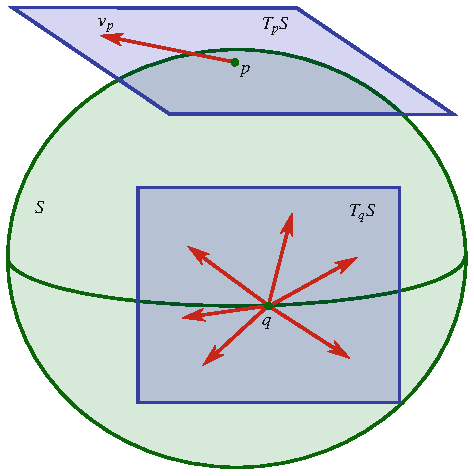
\includegraphics[width=0.562\linewidth]{images/vector/fig-10-2.pdf}
  \caption{向量 $v_p$，其中 $p$ 是``北极''. ``赤道''上点 $q$ 处的向量中有哪些与 $v_p$ 平行？}
  \label{fig:10-2}
\end{figure}

现在考虑图~\ref{fig:10-3} 所示的 $\mathbb{R}^2$ 中的点 $p$ 和 $q$. 关于两点之间的直线应该是什么样子，有一个非常自然且直观的想法. 而且，给定笛卡尔坐标系，我们知道如何测量两点之间的距离. 我们还知道环面 $T^2$ 是一个流形，因为 $T^2$ 的每个点的非常小的邻域看起来都像 $\mathbb{R}^2$. 然而，环面上点 $p$ 与 $q$ 之间的``直线''会是什么样子？在这种情形下``直线''究竟意味着什么？从图~\ref{fig:10-4} 中看不出这一点. 再退一步讲，人们如何测量环面上两点之间的距离？要回答这个问题，除了联络之外，还需要流形上一种称为\newterm{metric}{度量}{metric}的结构. 我们稍后实际上会多了解一点度量，不过不会深入. 总之，在一般流形上，我们必须显式地指定一个度量，而在欧几里得空间流形上，一个称为欧几里得度量的度量已经隐含地建立在我们对欧几里得空间的直观理解之中. 这是一般流形与我们熟悉的欧几里得空间流形 $\mathbb{R}^n$ 之间的另一个重大差别，也是我们必须谨慎区分两者的又一个原因.

\begin{figure}[htbp]
  \centering
  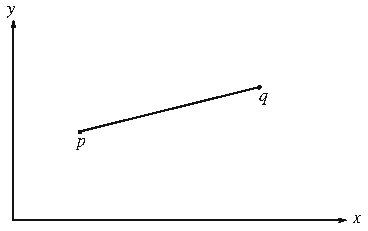
\includegraphics[width=0.436\linewidth]{images/vector/fig-10-3.pdf}
  \caption{流形 $\mathbb{R}^2$ 中两点 $p$ 与 $q$ 之间的一条直线. 直线在欧几里得空间中意味着什么是自然而直观的.}
  \label{fig:10-3}
\end{figure}

\begin{figure}[htbp]
  \centering
  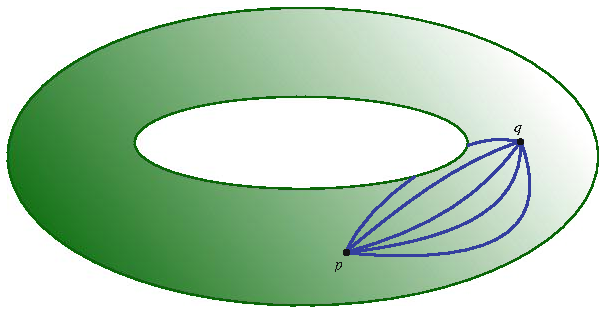
\includegraphics[width=0.721\linewidth]{images/vector/fig-10-4.pdf}
  \caption{环面 $T^2$，其上标出了两个点 $p$ 和 $q$. 图中画出了连接这两点的几条线. 连接流形 $T^2$ 上两点的``直线''会是什么样子？在这种情形下``直线''究竟意味着什么？}
  \label{fig:10-4}
\end{figure}

所有这一切都突显了一般流形与你所熟悉的欧几里得空间流形 $\mathbb{R}^n$ 之间的真正差别. 然而，在我们所做的一切中，我们都费了功夫区分``流形''$\mathbb{R}^n$ 与流形的切空间，后者基本上就是向量空间 $\mathbb{R}^n$. 既然你已经习惯了这一点，转向一般流形的情况应该不会太难.

现在我们准备给可微流形一个严格的定义. 在这里我们将坚持所谓的\newterm{differentiable-manifold}{微分流形}{differentiable manifold}. 实际上有很多不同类型的流形具有不同的性质. 由于这不是流形理论课程，我们将坚持最简单的那种. 一般流形保留欧几里得空间流形的一些结构，但不会保留欧几里得空间流形的联络或欧几里得度量.

\begin{definition}[$n$ 维流形]\label{def:10-1-1}
$n$ 维流形是一个空间 $M$，它可被一族局部\newterm{coordinate-neighborhood}{坐标邻域}{coordinate neighborhood} $U_i$ 连同一一映射 $\phi_i:U_i\to\mathbb{R}^n$ 完全覆盖，这些映射称为\newterm{coordinate-map}{坐标映射}{coordinate map}. $U_i$ 与 $\phi_i$ 合起来称为\newterm{coordinate-patch}{坐标片}{coordinate patch}或\newterm{chart}{坐标图}{chart}，一般记为 $(U_i,\phi_i)$. 所有坐标图合在一起 $\{(U_i,\phi_i)\}$ 称为 $M$ 的坐标系或\newterm{atlas}{图册}{atlas}. 由于 $U_i$ 覆盖整个 $M$，我们写 $M=\bigcup U_i$. 又因 $\phi_i$ 是一一的，它可逆，所以 $\phi_i^{-1}$ 存在且良定义. 最后，若两个坐标图有非空交集 $U_i\cap U_j\neq\emptyset$，则函数 $\phi_j\circ\phi_i^{-1}:\mathbb{R}^n\to\mathbb{R}^n$ 称为\newterm{transition-function}{转移函数}{transition function}.
\end{definition}

这里有很多重要的术语，我们总结如下：
\[
\begin{array}{rcl}
U_i & : & \text{坐标邻域},\\
\phi_i:U_i\to\mathbb{R}^n & : & \text{坐标映射},\\
(U_i,\phi_i) & : & \text{坐标片/坐标图},\\
\left\{(U_i,\phi_i)\right\} & : & \text{坐标系/图册},\\
\phi_j\circ\phi_i^{-1}:\mathbb{R}^n\to\mathbb{R}^n & : & \text{转移函数}.
\end{array}
\]

图~\ref{fig:10-5} 给出了一个二维的例子. 图册和坐标图这两个词尤其具有启发性；世界的图册（atlas）不就是一本地图（chart）的集合吗？这里 chart 一词是表示地图的航海用语.

\begin{figure}[htbp]
  \centering
  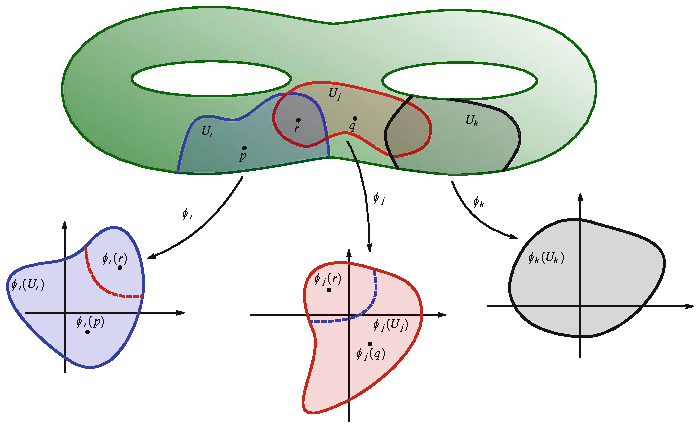
\includegraphics[width=0.960\linewidth]{images/vector/fig-10-5.pdf}
  \caption{这里展示了一个二维流形——双环面，连同三个坐标图 $(U_i,\phi_i)$、$(U_j,\phi_j)$ 和 $(U_k,\phi_k)$. 注意点 $r\in U_i\cap U_j$. 显然 $\phi_j\circ\phi_i^{-1}$ 把 $\phi_i(U_i\cap U_j)\subset\mathbb{R}^2$ 送到 $\phi_j(U_i\cap U_j)\subset\mathbb{R}^2$}
  \label{fig:10-5}
\end{figure}

现在考虑当点 $r\in U_i\cap U_j\neq\emptyset$ 时会发生什么. 我们有 $\phi_i(r)\in\mathbb{R}^n$ 和 $\phi_j(r)\in\mathbb{R}^n$. 此外，$\phi_j\circ\phi_i^{-1}$ 把 $\phi_i(U_i\cap U_j)\subset\mathbb{R}^n$ 送到 $\phi_j(U_i\cap U_j)\subset\mathbb{R}^n$，也就是说，$\phi_j\circ\phi_i^{-1}$ 是 $\mathbb{R}^n$ 的一个子集到 $\mathbb{R}^n$ 的另一个子集的映射，因此以 $\phi_i(U_i\cap U_j)$ 为定义域、以 $\phi_j(U_i\cap U_j)$ 为值域的映射 $\phi_j\circ\phi_i^{-1}:\mathbb{R}^n\to\mathbb{R}^n$，是我们知道如何从多元微积分求导的那种映射.

\begin{definition}[微分流形]\label{def:10-1-2}
微分流形是一个集合 $M$，连同坐标图族 $(U_i,\phi_i)$，其中 $M=\bigcup U_i$，使得每个映射 $\phi_j\circ\phi_i^{-1}$（其中 $U_i\cap U_j\neq\emptyset$）都是可微的.
\end{definition}

让我们看一个简单的显式例子，看看这是如何运作的. 考虑 $\mathbb{R}^2$ 中的单位圆 $S^1$. 我们将证明 $S^1$ 确实是一个微分流形. 令 $U_1$ 是 $S^1$ 中由 $0<t<2\pi$ 的点 $(\cos t,\sin t)$ 组成的子集. 那么由 $(\cos t,\sin t)\mapsto t$ 定义的 $\phi_1:U_1\to\mathbb{R}$ 是到开区间 $(0,2\pi)\subset\mathbb{R}$ 上的一一映射，所以 $(U_1,\phi_1)$ 是 $S^1$ 上的一个坐标图. 见图~\ref{fig:10-6}.

\begin{figure}[htbp]
  \centering
  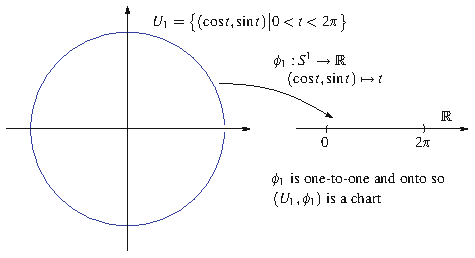
\includegraphics[width=0.582\linewidth]{images/vector/fig-10-6.pdf}
  \caption{$S^1$ 上的坐标图 $(U_1,\phi_1)$. $U_1$ 是 $S^1$ 中由 $0<t<2\pi$ 的点 $(\cos t,\sin t)$ 组成的子集，$\phi_1:U_1\to\mathbb{R}$ 由 $(\cos t,\sin t)\mapsto t$ 定义}
  \label{fig:10-6}
\end{figure}

类似地，令 $U_2$ 是 $S^1$ 中由 $-\pi<\tau<\pi$ 的点 $(\cos\tau,\sin\tau)$ 组成的子集. 那么由 $(\cos\tau,\sin\tau)\mapsto\tau$ 定义的 $\phi_2:U_2\to\mathbb{R}$ 是到 $\mathbb{R}$ 的某个子集上的一一映射，所以 $(U_2,\phi_2)$ 是 $S^1$ 上的另一个坐标图. 见图~\ref{fig:10-7}. 定义域 $U_1$ 和 $U_2$ 覆盖整个 $S^1$，即 $S^1=U_1\cup U_2$. 我们说 $(U_1,\phi_1)$ 和 $(U_2,\phi_2)$ 是 $S^1$ 的一个图册.

\begin{figure}[htbp]
  \centering
  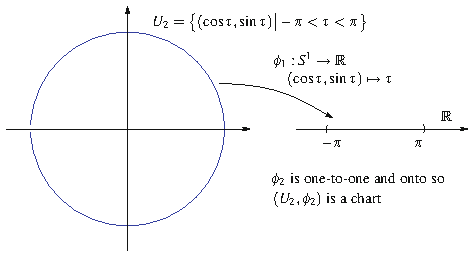
\includegraphics[width=0.582\linewidth]{images/vector/fig-10-7.pdf}
  \caption{$S^1$ 上的坐标图 $(U_2,\phi_2)$. $U_2$ 是 $S^1$ 中由 $-\pi<\tau<\pi$ 的点 $(\cos\tau,\sin\tau)$ 组成的子集，$\phi_2:U_2\to\mathbb{R}$ 由 $(\cos\tau,\sin\tau)\mapsto\tau$ 定义}
  \label{fig:10-7}
\end{figure}

\begin{question}\label{q:10-1}
$S^1$ 的哪个点不在 $U_1$ 中？$S^1$ 的哪个点不在 $U_2$ 中？为什么这些点没有被包含？它们能被包含进去吗？即使它们被包含进去了，仍然会出现什么问题？
\end{question}

注意 $U_1\cap U_2$ 有两个连通分支，即 $S^1$ 的上半开半圆和下半开半圆. 见图~\ref{fig:10-8}. 在上半开半圆上，对 $0<t<\pi$ 有 $\phi_1^{-1}\circ\phi_2(t)=t$，这是可微的；在下半开半圆上，对 $\pi<t<2\pi$ 有 $\phi_1^{-1}\circ\phi_2(t)=t-2\pi$，这也是可微的. 因此 $S^1$ 是一个微分流形.

\begin{figure}[htbp]
  \centering
  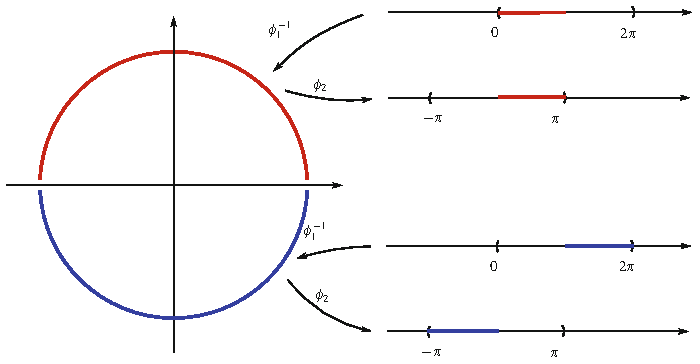
\includegraphics[width=0.867\linewidth]{images/vector/fig-10-8.pdf}
  \caption{$U_1\cap U_2$ 有两个连通分支：$S^1$ 的上半开半圆（红色）和下半开半圆（蓝色）. 在上半开半圆上，对 $0<t<\pi$ 有 $\phi_1^{-1}\circ\phi_2(t)=t$；在下半开半圆上，对 $\pi<t<2\pi$ 有 $\phi_1^{-1}\circ\phi_2(t)=t-2\pi$. 这两者都是可微的，使 $S^1$ 成为一个微分流形}
  \label{fig:10-8}
\end{figure}

在大多数微分几何教科书中，此时通常会出现可定向流形和带边流形的定义. 根据第 1.2 节你已经知道体积带有符号. 定向流形的思想与此相关，它本质上是指流形带有一种判断体积何时为正、何时为负的方式. 我们将在第 10.4 节讨论流形上的积分时讨论定向流形. 带边流形本质上就是你想象中的那种流形，即带有某种边界或``边缘''的流形. 什么是边界或``边缘''可以非常精确地用坐标图来定义. 在本书中我们不会显式地讨论带边流形，不过在第 11 章我们将在 Stokes 定理的具体语境中更仔细地探讨边界的某些概念.

\section{流形的切空间}

回想一下，我们之前引入切空间时，是通过考虑流形 $\mathbb{R}^n$ 来做的. 我们考虑的例子有 $n=2$ 或 $3$，但这个思想对任意 $n$ 都成立. 见图~\ref{fig:2-14} 至图~\ref{fig:2-17}. 我们选取一个点 $p\in\mathbb{R}^n$，然后考虑从该点出发的所有向量 $v_p$. 我们把从点 $p$ 出发的所有向量 $v_p$ 的集合称为 $\mathbb{R}^n$ 在 $p$ 处的切空间，记为 $T_p\mathbb{R}^n$. 然后我们看到 $T_p\mathbb{R}^n$ 本质上与向量空间 $\mathbb{R}^n$ 是同一个空间. 本节我们想给出切空间的一种稍微更抽象的表述.

例如，给定一个一般流形 $M$，你可能想知道我们说从点 $p\in M$ 发出的向量是什么意思. 毕竟，$\mathbb{R}^n$ 除了是微分流形之外，显然也是一个向量空间，这使我们能够谈论向量，而一般微分流形根本不需要是向量空间，这意味着流形中没有任何向量. 考虑图~\ref{fig:10-9} 所示的球面 $S^2\subset\mathbb{R}^3$. 我们可以在点 $p\in S^2$ 处画出各种各样与 $S^2$ 相切的向量，但这些向量实际上在空间 $\mathbb{R}^3$ 中——即流形 $S^2$ 所嵌入的空间——而不是在流形 $S^2$ 本身之中.

\begin{figure}[htbp]
  \centering
  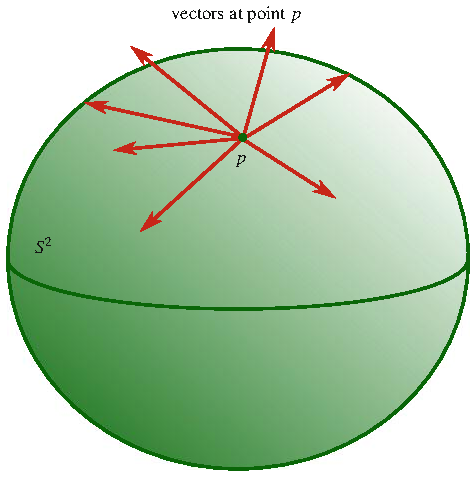
\includegraphics[width=0.564\linewidth]{images/vector/fig-10-9.pdf}
  \caption{流形 $S^2$ 连同点 $p$ 处若干个与 $S^2$ 相切的向量. 然而，这些向量实际上不在 $S^2$ 中. 它们事实上在 $\mathbb{R}^3$ 中，即我们为了画 $S^2$ 而把 $S^2$ 嵌入其中的那个空间}
  \label{fig:10-9}
\end{figure}

当我们最初引入切空间时，我们通过画几个流形并说点 $p$ 处的切空间本质上就是流形在该点的切平面（或超平面）来说明切空间的一般思想. 例如，图~\ref{fig:10-10} 中画出了流形 $S^2$ 连同它的几个切平面.

\begin{figure}[htbp]
  \centering
  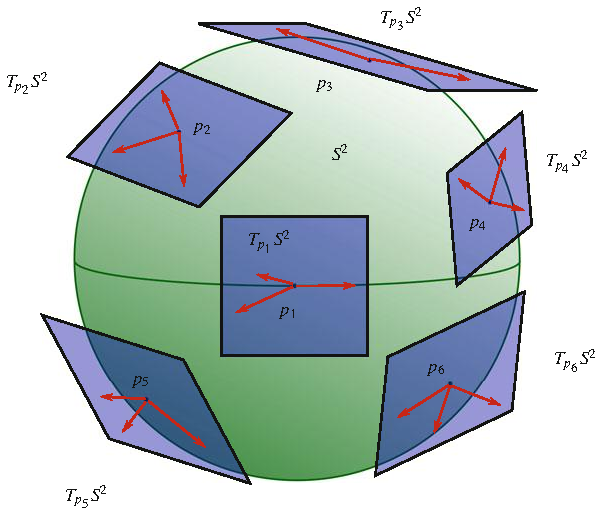
\includegraphics[width=0.850\linewidth]{images/vector/fig-10-10.pdf}
  \caption{当我们引入流形 $S^2$ 的切空间概念时，我们画出了流形在流形上各个点处的切平面. 实际上 $S^2$ 的每个点都有这样一个切平面}
  \label{fig:10-10}
\end{figure}

这是一个非常好的漫画式图画，有助于我们可视化和理解切空间，我们将继续使用它，但它要求我们的流形嵌入到某个 $\mathbb{R}^n$ 中，切空间也嵌入其中，就像 $S^2$ 和 $S^2$ 的切空间都嵌入 $\mathbb{R}^3$ 一样. 根据微分几何中一个深刻的定理——Whitney 嵌入定理，任何足够好的流形都可以嵌入到足够大的 $n$ 的 $\mathbb{R}^n$ 中，这意味着我们实际上可以继续使用我们的漫画式图画来帮助可视化和思考切空间. 然而，要以这种方式可视化切空间，我们实质上必须``走出''流形. 要求我们``走出''流形才能思考或定义它的性质称为\newterm{extrinsic-property}{外蕴性质}{extrinsic property}.

\begin{figure}[htbp]
  \centering
  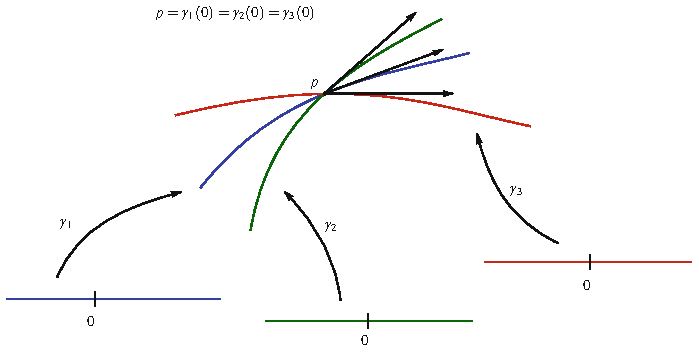
\includegraphics[width=0.865\linewidth]{images/vector/fig-10-11.pdf}
  \caption{三条曲线 $\gamma_i:(-\epsilon,\epsilon)\subset\mathbb{R}\longrightarrow M$（$i=1,2,3$），使得 $\gamma_i(0)=p$. 每条曲线在点 $p$ 处都有一个切向量}
  \label{fig:10-11}
\end{figure}

我们希望能够在不必``走出''流形的情况下定义和思考切空间. 在很多情况下，能够``留在流形内部''思考流形的性质是有用的. 我们可以在``留在流形内部''的同时定义或思考的流形性质称为\newterm{intrinsic-property}{内蕴性质}{intrinsic property}. 内蕴性质绝不需要或依赖于流形嵌入到某个 $\mathbb{R}^n$ 中. 尽管到目前为止我们一直在从外蕴的角度思考切向量和切空间，但它们实际上是内蕴性质. 我们可以在``留在流形内部''的同时定义它们和思考它们. 当我们这样做时，从点发出的箭头的想法就不再合适了.

我们将通过首先考虑所有满足 $\gamma(0)=p\in M$ 的\newterm{smooth-curve}{光滑曲线}{smooth curve}
\[
\gamma:(-\epsilon,\epsilon)\subset\mathbb{R}\longrightarrow M
\]
来接近切向量的内蕴定义，其中 $\epsilon$ 只是某个小的正数. 在图~\ref{fig:10-11} 中我们画了几条光滑曲线 $\gamma_i:(-\epsilon,\epsilon)\to M$，其中对所有 $i$ 都有 $\gamma_i(0)=p$. 我们把 $\gamma_i$ 所依赖的参数称为时间. 不去深究光滑曲线的技术含义，只需假定它意味着你直观上认为的那个意思，即曲线上没有尖角.

每个切向量 $v_p$ 实际上都与某条经过点 $p\in M$ 的光滑曲线相切. 但是，虽然切向量 $v_p$ 可能实际上只存在于 $M$ 所嵌入的空间 $\mathbb{R}^n$ 中，曲线 $\gamma$ 却完全存在于流形 $M$ 之中. 本质上，这些曲线中的每一条都在点 $p$ 处定义了一个不同的切向量. 因此，一般的思想是把流形 $M$ 在点 $p$ 处的切向量与流形中经过点 $p$ 的曲线等同起来，从而不再需要把 $M$ 嵌入到某个更大的空间 $\mathbb{R}^n$ 中就能拥有切向量.

看起来似乎 $M$ 的切空间可能等价于满足 $\gamma(0)=p$ 的曲线 $\gamma:(-\epsilon,\epsilon)\to M$ 的集合. 这几乎是对的，但不完全对. 有两个问题我们必须仔细考虑. 为处理第一个问题，考虑图~\ref{fig:10-12}. 这里有三条不同的曲线 $\gamma_1,\gamma_2,\gamma_3:(-\epsilon,\epsilon)\to M$，满足 $\gamma_1(0)=\gamma_2(0)=\gamma_3(0)=p$，它们在非常靠近 $p$ 的地方是相同的. 如果两条曲线在非常靠近 $p$ 的地方是相同的，那么我们能否在某种意义下认为它们是同一条曲线？乍一看这样做似乎是合理的.

\begin{figure}[htbp]
  \centering
  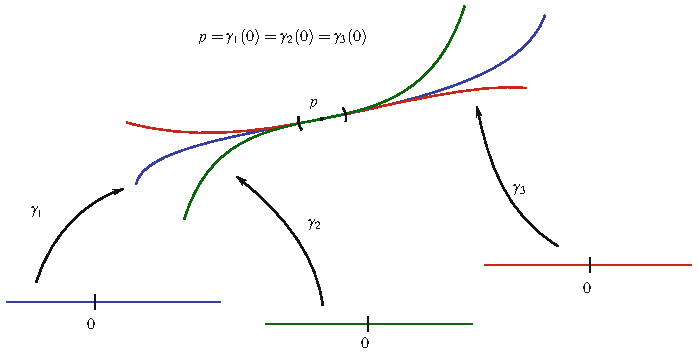
\includegraphics[width=0.829\linewidth]{images/vector/fig-10-12.pdf}
  \caption{与图~\ref{fig:10-11} 一样，三条曲线 $\gamma_i:(-\epsilon,\epsilon)\subset\mathbb{R}\longrightarrow M$（$i=1,2,3$），使得 $\gamma_i(0)=p$. 不过，这里当我们非常靠近 $p$ 时，这些曲线是相同的}
  \label{fig:10-12}
\end{figure}

为考虑第二个问题，考虑 $T_pM$ 中的向量 $v_p$ 和 $2v_p$. 从图~\ref{fig:10-13} 来看，$v_p$ 和 $2v_p$ 都可以由同一条曲线 $\gamma$ 表示. 问题是，当我们使用曲线时，如何区分 $T_pM$ 中的向量 $v_p$ 和 $2v_p$？它们指向相同的方向，但第二个向量是第一个向量的两倍长.

\begin{figure}[htbp]
  \centering
  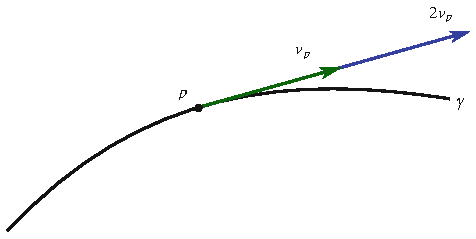
\includegraphics[width=0.564\linewidth]{images/vector/fig-10-13.pdf}
  \caption{两个向量 $v_p$ 和 $2v_p$，它们看起来都与同一条曲线 $\gamma$ 相切}
  \label{fig:10-13}
\end{figure}

处理这第二个问题的线索在于，我们把 $\gamma$ 所依赖的参数称为时间. $\gamma$ 在时间 $t=0$ 处的导数给出时间 $0$ 处的速度. 当我们提高沿曲线 $\gamma$ 运动的速率时，速度更大，因而速度向量变得更长. 因此，为了区分 $v_p$ 和 $2v_p$，参数化的速度被提高，使其在 $t=0$ 处是原来的两倍.

让我们考虑一个简单的例子. 令 $M=\mathbb{R}_{xy}^2$ 为以 $x$ 和 $y$ 参数化的欧几里得平面. 考虑 $\mathbb{R}_{xy}^2$ 的原点处的下列三个向量：
\[
u_0=\binom{1}{2},\qquad v_0=2u_0=\binom{2}{4},\qquad w_0=-u_0=\binom{-1}{-2}.
\]

见图~\ref{fig:10-14}. 这些向量由下列三条曲线 $\alpha,\beta,\gamma:(-\epsilon,\epsilon)\to\mathbb{R}_{xy}^2$ 给出，其中
\[
\begin{aligned}
\alpha(t)&=\bigl(\alpha_1(t),\alpha_2(t)\bigr)=(t,2t),\\
\beta(t)&=\bigl(\beta_1(t),\beta_2(t)\bigr)=(2t,4t),\\
\gamma(t)&=\bigl(\gamma_1(t),\gamma_2(t)\bigr)=(-t,-2t).
\end{aligned}
\]

尽管在 $\mathbb{R}^2$ 中画出曲线 $\alpha$、$\beta$ 和 $\gamma$ 看起来像是同一条曲线，严格地说它们都是不同的曲线，因为它们的参数化不同.

\begin{figure}[htbp]
  \centering
  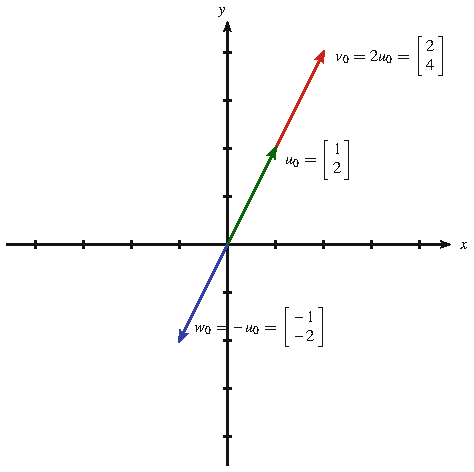
\includegraphics[width=0.562\linewidth]{images/vector/fig-10-14.pdf}
  \caption{流形 $\mathbb{R}_{xy}^2$，原点处有三个向量 $u_0=[1,2]^T$、$v_0=2u_0=[2,4]^T$ 和 $w_0=-u_0=[-1,-2]^T$. 这三个向量由具有不同参数化的三条曲线 $\alpha$、$\beta$ 和 $\gamma$ 确定}
  \label{fig:10-14}
\end{figure}

现在我们将用 $M$ 上的曲线来定义 $M$ 在点 $p$ 处的切空间 $T_pM$，但我们必须把上述两个问题考虑进去. 如图~\ref{fig:10-12} 那样，在非常靠近 $p$ 的地方相同的两条曲线，在靠近 $p$ 的地方有相同的值域. 如果两条曲线在靠近 $p$ 处有相同的值域，并且在靠近 $p$ 处有相同的参数化，则称它们等价，记为 $\sim$. 假设 $\gamma_1$、$\gamma_2$ 和 $\gamma_3$ 在靠近 $p$ 处都有相同的值域，并且在靠近 $p$ 处都有相同的参数化，那么我们说 $\gamma_1\sim\gamma_2\sim\gamma_3$.

\begin{definition}[曲线的等价类]\label{def:10-2-1}
所有等价曲线的集合称为\newterm{equivalence-class}{等价类}{equivalence class}. $\gamma_1$ 的等价类是与 $\gamma_1$ 等价的所有曲线的集合，记为 $[\gamma_1]$，定义为
\[
[\gamma_1]\equiv\left\{\gamma\mid\gamma\sim\gamma_1\right\}.
\]
\end{definition}

因此，若 $\gamma_1\sim\gamma_2\sim\gamma_3$，则有 $[\gamma_1]=[\gamma_2]=[\gamma_3]$. 这意味着用等价类中的哪个成员来表示该等价类并不重要.

\begin{definition}[切空间]\label{def:10-2-2}
点 $p$ 处曲线的每个等价类被定义为 $p$ 处的一个切向量. 当我们想指出基点是 $p$ 时，我们写 $[\gamma]_p$. $M$ 在 $p$ 处的切空间被定义为点 $p$ 处所有切向量（即曲线的等价类）的集合，
\[
T_pM=\left\{[\gamma]_p\mid\gamma:(-\epsilon,\epsilon)\to M\text{ 且 }\gamma(0)=p\right\}.
\]
\end{definition}

因此，流形 $M$ 在点 $p$ 处的切空间是经过 $p\in M$ 的所有曲线的等价类的集合. 注意，切空间的这个定义是内蕴的，它完全依赖于流形 $M$ 中经过点 $p$ 的曲线. 因此我们不需要``走出''流形就能可视化或思考切空间. 这个定义独立于我们的流形所嵌入的任何更大的空间.

现在我们要理解向量的外蕴观点与内蕴观点之间的关系. 实际位于我们的流形所嵌入的空间中的向量 $v_p$，是某条曲线 $\gamma$ 在点 $p$ 处的速度向量，所以我们做了等同 $v_p=[\gamma]_p$. 要从曲线 $\gamma$ 重新得到向量 $v_p$，我们必须对时间求 $\gamma$ 的导数，并在时间 $t=0$ 处求值. 基本上，我们是在求映射 $\gamma:(-\epsilon,\epsilon)\to M$ 的 Jacobian 矩阵.

回到我们的具体例子，我们有
\[
u_{(0,0)}\equiv[\alpha]_{(0,0)},\qquad v_{(0,0)}\equiv[\beta]_{(0,0)},\qquad w_{(0,0)}\equiv[\gamma]_{(0,0)}.
\]

但请注意，尽管当我们把曲线画在 $\mathbb{R}^2$ 上时，它们在我们的图画中看起来都是``同一条''曲线，但它们实际上是不同的曲线，因为它们的参数化不同，所以不属于同一个曲线等价类. 换言之，我们有 $\alpha\nsim\beta$、$\alpha\nsim\gamma$ 和 $\beta\nsim\gamma$. 通常我们只简单地用 $0$ 表示基点 $(0,0)$，但由于我们想强调基点与在时间 $t=0$ 处对偏导数求值之间的区别，这里我们要对记号格外小心. 我们可以看到我们关于向量的两种观点是如何相互关联的，
\begin{align*}
u_{(0,0)}\equiv\left[\left(\alpha_1(t),\alpha_2(t)\right)\right]_{(0,0)}=\left[(t,2t)\right]_{(0,0)}, \\
u_{(0,0)}=\begin{bmatrix}\left.\dfrac{\partial\alpha_1(t)}{\partial t}\right|_{t=0}\\[1.2em] \left.\dfrac{\partial\alpha_2(t)}{\partial t}\right|_{t=0}\end{bmatrix}_{(0,0)}=\begin{bmatrix}\left.\dfrac{\partial(t)}{\partial t}\right|_{t=0}\\[1.2em] \left.\dfrac{\partial(2t)}{\partial t}\right|_{t=0}\end{bmatrix}_{(0,0)}=\binom{1}{2}_{(0,0)}.
\end{align*}
类似地，我们有
\begin{align*}
v_{(0,0)}\equiv\left[\left(\beta_1(t),\beta_2(t)\right)\right]_{(0,0)}=\left[(2t,4t)\right]_{(0,0)}, \\
v_{(0,0)}=\begin{bmatrix}\left.\dfrac{\partial\beta_1(t)}{\partial t}\right|_{t=0}\\[1.2em] \left.\dfrac{\partial\beta_2(t)}{\partial t}\right|_{t=0}\end{bmatrix}_{(0,0)}=\begin{bmatrix}\left.\dfrac{\partial(2t)}{\partial t}\right|_{t=0}\\[1.2em] \left.\dfrac{\partial(4t)}{\partial t}\right|_{t=0}\end{bmatrix}_{(0,0)}=\binom{2}{4}_{(0,0)},
\end{align*}
以及
\begin{align*}
w_{(0,0)}\equiv\left[\left(\gamma_1(t),\gamma_2(t)\right)\right]_{(0,0)}=\left[(-t,-2t)\right]_{(0,0)}, \\
w_{(0,0)}=\begin{bmatrix}\left.\dfrac{\partial\gamma_1(t)}{\partial t}\right|_{t=0}\\[1.2em] \left.\dfrac{\partial\gamma_2(t)}{\partial t}\right|_{t=0}\end{bmatrix}_{(0,0)}=\begin{bmatrix}\left.\dfrac{\partial(-t)}{\partial t}\right|_{t=0}\\[1.2em] \left.\dfrac{\partial(-2t)}{\partial t}\right|_{t=0}\end{bmatrix}_{(0,0)}=\binom{-1}{-2}_{(0,0)}.
\end{align*}

下面是我们在流形上定义向量的两种方式之间进行转换的钥匙. 等价类定义基于完全存在于我们的流形 $M$ 内部的曲线，不需要把 $M$ 嵌入到更大的环境空间就能``看到''向量；我们的向量只是被看作完全位于 $M$ 中的曲线. 我在这里将称之为向量定义的方式，需要把我们的流形 $M$ 嵌入到环境空间 $\mathbb{R}^n$ 中，或者在一点处画出流形 $M$ 的切空间，才能``看到''向量. 在等价类定义中，我们把曲线看作向量；在向量定义中，我们把曲线的导数看作向量. 这在你看来可能很奇怪，但这只是从两个不同的视角思考向量而已. 希望这不会太令人困惑.

\[
\begin{array}{c|c|c}
\hline
\text{等价类定义} & \Longleftrightarrow & \underline{\text{向量定义}}\\
\hline
v_p=[\gamma]_p,\quad p=\gamma(0) & & v_p=[\gamma']_p=[\gamma]_p'\\
=\left[\left(\gamma_1(t),\ldots,\gamma_n(t)\right)\right] & & =\left[\left(\gamma_1'(t),\ldots,\gamma_n'(t)\right)\right]_p\\
& & =\left[\left(\gamma_1(t),\ldots,\gamma_n(t)\right)\right]_p'\\
& & =\begin{bmatrix}\gamma_1'(t=0)\\ \vdots\\ \gamma_n'(t=0)\end{bmatrix}_p\\
& & =\begin{bmatrix}\left.\dfrac{\partial\gamma_1(t)}{\partial t}\right|_{t=0}\\[1.2em] \vdots\\[0.6em] \left.\dfrac{\partial\gamma_n(t)}{\partial t}\right|_{t=0}\end{bmatrix}_p\\
\hline
\end{array}
\]

这里还要再说一句. 如我们所知，积分在某种意义上与微分相反. 如果我们能把向量 $v_p$ 看作曲线 $\gamma$ 在点 $p$ 处的导数，那么我们能否把曲线 $\gamma$ 看作向量 $v_p$ 的积分？这里的问题是 $v_p$ 只存在于单独一个点处，而在一个点处积分的想法是定义不清的. 为了做积分，我们需要在某个点周围有一个光滑向量场. 不去深究光滑向量场的技术细节，把它想成一个随着点变化而光滑变化的向量场即可. 一旦我们在某个邻域中有了一个光滑向量场，我们就可以谈论称为积分曲线的曲线了. 用来表示某个向量 $v_p$ 的等价类 $[\gamma]_p$ 的曲线 $\gamma$ 不必是积分曲线，但如果 $v_p$ 是光滑向量场的一个元素，那么人们通常会做出一个未言明的假设：$\gamma$ 是一条积分曲线. 我们将在第 12 章和附录 B 中在电磁学和几何力学的语境下更详细地讨论积分曲线.

回想一下，在第 2.3 节中，我们把点 $p$ 处的切向量与方向导数等同起来. 通过这样做，我们把切空间的欧几里得基向量与偏微分算子等同起来. 换言之，我们找到了下列等同，
\[
e_{1p}=\left.\frac{\partial}{\partial x}\right|_p,\qquad e_{2p}=\left.\frac{\partial}{\partial y}\right|_p,\qquad e_{3p}=\left.\frac{\partial}{\partial z}\right|_p.
\]

因此，对于向量 $v_p\in T_p\mathbb{R}^3$，
\[
v_p=\begin{bmatrix}v_1\\v_2\\v_3\end{bmatrix}_p=v_1e_{1p}+v_2e_{2p}+v_3e_{3p}=v_1\left.\frac{\partial}{\partial x}\right|_p+v_2\left.\frac{\partial}{\partial y}\right|_p+v_3\left.\frac{\partial}{\partial z}\right|_p.
\]

考虑 $\gamma:(-\epsilon,\epsilon)\to M$（其中 $\gamma(0)=p$）和 $f:M\to\mathbb{R}$. 那么 $f\circ\gamma:(-\epsilon,\epsilon)\subset\mathbb{R}\to\mathbb{R}$，如图~\ref{fig:10-15} 所示. 函数 $f:\mathbb{R}^3\to\mathbb{R}$ 在方向 $v_p$ 上的方向导数被写为向量 $v_p$ 作用在函数 $f$ 上，
\[
v_p[f]=\left(v_1\left.\frac{\partial}{\partial x}\right|_p+v_2\left.\frac{\partial}{\partial y}\right|_p+v_3\left.\frac{\partial}{\partial z}\right|_p\right)[f]=v_1\left.\frac{\partial f}{\partial x}\right|_p+v_2\left.\frac{\partial f}{\partial y}\right|_p+v_3\left.\frac{\partial f}{\partial z}\right|_p.
\]

\begin{figure}[htbp]
  \centering
  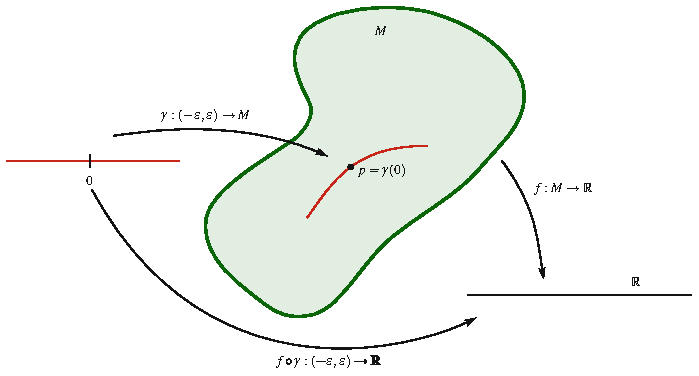
\includegraphics[width=0.960\linewidth]{images/vector/fig-10-15.pdf}
  \caption{由 $\gamma:(-\epsilon,\epsilon)\to M$（其中 $\gamma(0)=p$）给出的向量 $[\gamma]_p$ 以及函数 $f:M\to\mathbb{R}$. 于是有 $f\circ\gamma:(-\epsilon,\epsilon)\subset\mathbb{R}\to\mathbb{R}$，这是我们知道如何求导的那种映射}
  \label{fig:10-15}
\end{figure}

我们想在更抽象的、向量 $v_p$ 由曲线等价类 $[\gamma]_p$ 给出的内蕴背景中考虑这是什么，即当我们有 $v_p\equiv[\gamma]_p$ 时. 以前我们用记号 $v_p[f]$ 表示 $D_{v_p}f$，即 $f$ 在 $v_p$ 方向上的方向导数. 我们用这个记号来强调这样一个事实：在某种意义上，正是向量 $v_p$ 在作用在函数 $f$ 上. 只要我们把向量写成 $v_p$，我们就继续使用这个记号；但当我们用曲线等价类记号 $[\gamma]_p$ 写向量时，写 $[\gamma]_p[f]$ 就有点奇怪了，因为两组方括号 $[\cdot]$ 有不同的含义. 记号有时与习惯和约定一样多的是理性规划的结果.

当我们的向量 $v_p$ 由曲线等价类 $[\gamma]_p$ 给出时，$f$ 在 $v_p$ 方向上的方向导数由下式给出，
\[
\begin{aligned}
v_p[f]=D_{[\gamma]_p}f&=[f\circ\gamma]_p'\\
&=\left.\frac{\partial(f\circ\gamma)}{\partial t}\right|_{t=0}\\
&=\lim_{h\to 0}\frac{(f\circ\gamma)(h)-(f\circ\gamma)(0)}{h}.
\end{aligned}
\]

一个常用的记号是 $D_{[\gamma]_p}f$，它模仿多元微积分中通常使用的记号. $D_{[\gamma]_p}f$ 的其他记号包括 $[(f\circ\gamma)']_p$、$[f\circ\gamma]_p'$、$[(f\circ\gamma)']_{t=0}$ 甚至 $[f\circ\gamma]_{t=0}'$. 没有一种完全标准的写法，你可以在记号中使用各种不同的变体. 当然关键之处在于，如果向量在点 $p=\gamma(0)$ 处，那就意味着 $\gamma$ 的导数必须在 $t=0$ 处求值. 这才是要点. 此外，通常人们只写一个 $0$. 你需要根据语境来判断 $0$ 是指在 $t=0$ 处求值，还是基点是原点 $(0,0)$. 发出这个警告之后，我们就不再试图如此精确了.

注意，$f$ 在点 $p=\gamma(0)$ 处沿方向 $[\gamma]_p$ 的方向导数被定义为与一元函数 $f\circ\gamma$ 在 $t=0$ 处的普通导数相同的东西. 很容易看出，用这个记号我们会得到相同的答案. 假设 $\gamma(t)=\bigl(x(t),y(t),z(t)\bigr)$，于是有
\[
v_p=\left[\bigl(x(t),y(t),z(t)\bigr)\right]_p'=\begin{bmatrix}x'(t=0)\\ y'(t=0)\\ z'(t=0)\end{bmatrix}_p.
\]
利用 $f\circ\gamma(t)=f\bigl(x(t),y(t),z(t)\bigr)$，我们进而得到
\[
\begin{aligned}
v_p[f]=D_{[\gamma]_p}f&=\left.\frac{\partial(f\circ\gamma)}{\partial t}\right|_{t=0}\\
&=\left.\frac{\partial f\bigl(x(t),y(t),z(t)\bigr)}{\partial t}\right|_0\\
&=\left.\frac{\partial f}{\partial x}\right|_{\gamma(0)}\cdot\left.\frac{\partial x}{\partial t}\right|_0+\left.\frac{\partial f}{\partial y}\right|_{\gamma(0)}\cdot\left.\frac{\partial y}{\partial t}\right|_0+\left.\frac{\partial f}{\partial z}\right|_{\gamma(0)}\cdot\left.\frac{\partial z}{\partial t}\right|_0\qquad\text{链式法则}\\
&=\left.\frac{\partial f}{\partial x}\right|_p\underbrace{x'(0)}_{v_1}+\left.\frac{\partial f}{\partial y}\right|_p\underbrace{y'(0)}_{v_2}+\left.\frac{\partial f}{\partial z}\right|_p\underbrace{z'(0)}_{v_3},
\end{aligned}
\]
这与上面我们得到的 $v_p[f]$ 完全一样，只是记号中去掉了基点 $p$.

回到一个具体的例子，假设我们有函数 $f:\mathbb{R}_{xy}^2\to\mathbb{R}$，由 $f(x,y)=x+\sin(y)$ 给出. 我们想求 $u_0[f]$，其中 $u_0=\binom{1}{2}=[(t,2t)]_0$. （注意，这里我们有 $0=(0,0)$.）像以前那样进行，我们有
\[
\begin{aligned}
u_0[f]&=\left(1\cdot\left.\frac{\partial}{\partial x}\right|_0+2\cdot\left.\frac{\partial}{\partial y}\right|_0\right)f\\
&=1\cdot\left.\frac{\partial\bigl(x+\sin(y)\bigr)}{\partial x}\right|_0+2\cdot\left.\frac{\partial\bigl(x+\sin(y)\bigr)}{\partial y}\right|_0\\
&=1\cdot 1+2\cdot\cos(0)\\
&=3.
\end{aligned}
\]
然而，用 $u_0=[\gamma]_0=\left[(t,2t)\right]_0$，我们有
\[
\begin{aligned}
D_{u_0}f=[f\circ\gamma]_0'&=\left.\frac{\partial(f\circ\gamma)}{\partial t}\right|_0\\
&=\left.\frac{\partial\bigl(t+\sin(2t)\bigr)}{\partial t}\right|_0\\
&=\left.1+2\cos(2t)\right|_0\\
&=1+2=3.
\end{aligned}
\]

这一切看起来都很好，直到你注意到在我们的例子中，我们的流形是 $\mathbb{R}_{xy}^2$，即``内置''了笛卡尔坐标系的 $\mathbb{R}^2$. 求复合 $f\circ\gamma$ 依赖于知道这个坐标系. 为什么？因为函数 $f$ 是显式地用变量 $x$ 和 $y$ 写出来的，这使得写出 $f\circ\gamma$ 很容易. 但是在一个没有``内置''很好标准坐标系的流形上，我们如何处理方向导数呢？换言之，如果写出 $f\circ\gamma$ 实际上是什么并不那么直截了当，那该怎么办？

如果我们想求 $f:M\to\mathbb{R}$ 在点 $p\in M$ 处沿方向 $v_p\equiv[\gamma]_p$ 的导数，那么我们需要知道如何复合 $f$ 和 $\gamma$，得到映射 $f\circ\gamma:(-\epsilon,\epsilon)\subset\mathbb{R}\to\mathbb{R}$. 但对于任意流形 $M$，这实际上可能并不清楚. 复合 $f\circ\gamma$ 实际上依赖于某个坐标图 $\phi$. 因此，我们的复合 $f\circ\gamma$ 必须借助某个坐标图来完成，以便我们能处理从 $\mathbb{R}^n$ 到 $\mathbb{R}^m$ 的映射，这是我们理解的. 考虑图~\ref{fig:10-16}. 由于微分流形带有坐标图 $(U,\phi)$，我们可以利用它们. 我们有
\[
f\circ\gamma=f\circ\phi^{-1}\circ\phi\circ\gamma.
\]

\begin{figure}[htbp]
  \centering
  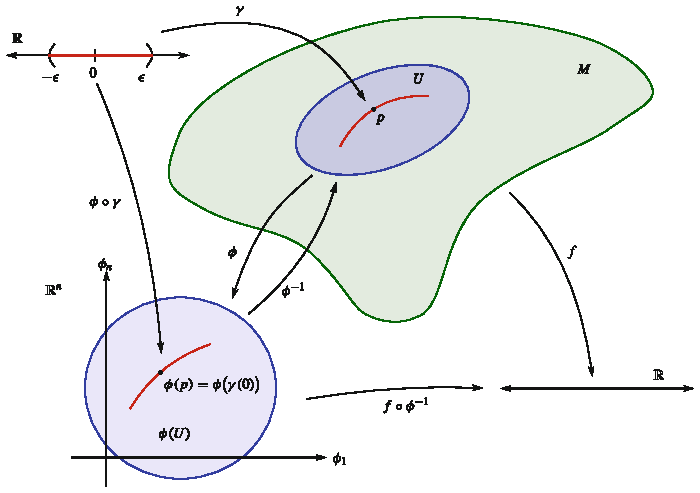
\includegraphics[width=0.960\linewidth]{images/vector/fig-10-16.pdf}
  \caption{这里展示了流形 $M$ 以及三样东西：(a) 表示点 $p$ 处切向量的曲线 $\gamma$，(b) 流形 $M$ 上的实值函数 $f:M\to\mathbb{R}$，(c) 满足 $p\in U$ 的坐标图 $(U,\phi)$. 显然有 $f\circ\gamma=f\circ\phi^{-1}\circ\phi\circ\gamma=(f\circ\phi^{-1})\circ(\phi\circ\gamma)$. 图中还画出了映射 $\phi\circ\gamma:\mathbb{R}\to\mathbb{R}^n$ 和 $f\circ\phi^{-1}:\mathbb{R}^n\to\mathbb{R}$}
  \label{fig:10-16}
\end{figure}

映射 $\phi\circ\gamma:(-\epsilon,\epsilon)\subset\mathbb{R}\to\phi(U)\subset\mathbb{R}^n$ 是我们实际上可以计算并求导的那种映射，映射 $f\circ\phi^{-1}:\phi(U)\subset\mathbb{R}^n\to\mathbb{R}$ 也是如此. 所以我们实际上有
\[
\begin{aligned}
v_p[f]=D_{[\gamma]_p}f&=[f\circ\gamma]_0'\\
&=[f\circ\phi^{-1}\circ\phi\circ\gamma]_0'\\
&=[f\circ\phi^{-1}]_{\phi(p)}'\cdot[\phi\circ\gamma]_0'\\
&=\left.\frac{\partial(f\circ\phi^{-1})}{\partial\phi}\right|_{\phi(p)}\cdot\left.\frac{\partial(\phi\circ\gamma)}{\partial t}\right|_0.
\end{aligned}
\]

注意我们得到
\begin{center}
\fbox{\parbox{0.92\textwidth}{\centering
曲线情形的链式法则：\\[0.4em]
$[f\circ\phi^{-1}\circ\phi\circ\gamma]_0'=[f\circ\phi^{-1}]_{\phi\circ\gamma(0)}'\cdot[\phi\circ\gamma]_0'=[f\circ\phi^{-1}]_{\phi(p)}'\cdot[\phi\circ\gamma]_0'.$
}}
\end{center}

这实际上就是链式法则的一种写法. 它看起来可能一点也不像你习惯的链式法则，但这就是链式法则在这个语境中的样子——当我们使用向量的曲线等价类定义来求导时.

为证明这一点，让我们分别考虑这些项中的每一项. 首先我们来看映射
\[
\begin{array}{c}
\phi\circ\gamma:(-\epsilon,\epsilon)\subset\mathbb{R}\longrightarrow\phi(U)\subset\mathbb{R}^n\\
t\longmapsto\Bigl(\phi_1\bigl(\gamma(t)\bigr),\phi_2\bigl(\gamma(t)\bigr),\ldots,\phi_n\bigl(\gamma(t)\bigr)\Bigr)\\
=\Bigl(\phi_1\circ\gamma(t),\phi_2\circ\gamma(t),\ldots,\phi_n\circ\gamma(t)\Bigr)
\end{array}
\]
所以 $\left.\frac{\partial(\phi\circ\gamma)}{\partial t}\right|_0$ 实际上是在 $t=0$ 处求值的 Jacobian 矩阵，
\[
\left.\frac{\partial(\phi\circ\gamma)}{\partial t}\right|_0=\begin{bmatrix}\left.\dfrac{\partial(\phi_1\circ\gamma)}{\partial t}\right|_0\\[1.2em] \left.\dfrac{\partial(\phi_2\circ\gamma)}{\partial t}\right|_0\\[1.2em] \vdots\\[0.6em] \left.\dfrac{\partial(\phi_n\circ\gamma)}{\partial t}\right|_0\end{bmatrix}.
\]

接下来我们来看映射
\[
\begin{array}{c}
f\circ\phi^{-1}:\phi(U)\subset\mathbb{R}^n\longrightarrow\mathbb{R}\\
(\phi_1,\phi_2,\ldots,\phi_n)\longmapsto f\bigl(\phi^{-1}(\phi_1,\phi_2,\ldots,\phi_n)\bigr)\\
=f\circ\phi^{-1}(\phi_1,\phi_2,\ldots,\phi_n)
\end{array}
\]
所以 $\left.\frac{\partial(f\circ\phi^{-1})}{\partial\phi}\right|_{\phi(p)}$ 实际上是在 $\phi(p)$ 处求值的 Jacobian 矩阵，
\[
\left.\frac{\partial(f\circ\phi^{-1})}{\partial\phi}\right|_{\phi(p)}=\left[\left.\frac{\partial(f\circ\phi^{-1})}{\partial\phi_1}\right|_{\phi(p)},\left.\frac{\partial(f\circ\phi^{-1})}{\partial\phi_2}\right|_{\phi(p)},\ldots,\left.\frac{\partial(f\circ\phi^{-1})}{\partial\phi_n}\right|_{\phi(p)}\right].
\]

把这两部分合在一起，我们有
\[
\begin{aligned}
D_{[\gamma]_p}f&=\left[\left.\frac{\partial(f\circ\phi^{-1})}{\partial\phi_1}\right|_{\phi(p)},\left.\frac{\partial(f\circ\phi^{-1})}{\partial\phi_2}\right|_{\phi(p)},\ldots,\left.\frac{\partial(f\circ\phi^{-1})}{\partial\phi_n}\right|_{\phi(p)}\right]\begin{bmatrix}\left.\dfrac{\partial(\phi_1\circ\gamma)}{\partial t}\right|_0\\[1.2em] \left.\dfrac{\partial(\phi_2\circ\gamma)}{\partial t}\right|_0\\[1.2em] \vdots\\[0.6em] \left.\dfrac{\partial(\phi_n\circ\gamma)}{\partial t}\right|_0\end{bmatrix}\\
&=\left.\frac{\partial(f\circ\phi^{-1})}{\partial\phi_1}\right|_{\phi(p)}\left.\frac{\partial(\phi_1\circ\gamma)}{\partial t}\right|_0+\cdots+\left.\frac{\partial(f\circ\phi^{-1})}{\partial\phi_n}\right|_{\phi(p)}\left.\frac{\partial(\phi_n\circ\gamma)}{\partial t}\right|_0\\
&=\sum_{i=1}^{n}\left.\frac{\partial(f\circ\phi^{-1})}{\partial\phi_i}\right|_{\phi(p)}\left.\frac{\partial(\phi_i\circ\gamma)}{\partial t}\right|_0.
\end{aligned}
\]

还要注意，这意味着
\[
[f\circ\phi^{-1}]_{\phi(p)}'\cdot[\phi\circ\gamma]_0'=\sum_{i=1}^{n}\left.\frac{\partial(f\circ\phi^{-1})}{\partial\phi_i}\right|_{\phi(p)}\left.\frac{\partial(\phi_i\circ\gamma)}{\partial t}\right|_0,
\]
这清楚地表明 $[f\circ\phi^{-1}]_{\phi(p)}'\cdot[\phi\circ\gamma]_0'$ 确实只是链式法则的另一种写法.

\begin{question}\label{q:10-2}
假设 $(U,\phi)$ 和 $(\widetilde{U},\widetilde{\phi})$ 是 $M$ 上的两个坐标图，$p\in U\cap\widetilde{U}$，$\gamma:(-\epsilon,\epsilon)\subset\mathbb{R}\to M$ 满足 $\gamma(0)=p$，且 $f$ 是 $M$ 上的实值函数. 证明
\[
\left.\frac{\partial(f\circ\phi^{-1}\circ\phi\circ\gamma)}{\partial t}\right|_0=\left.\frac{\partial(f\circ\widetilde{\phi}^{-1}\circ\widetilde{\phi}\circ\gamma)}{\partial t}\right|_0.
\]
\end{question}

\section{流形上的前推与拉回}

我们在第 6 章已经讨论过前推和拉回. 我们仔细考察过的例子之一是变量替换公式 $f:\mathbb{R}_{xy}^2\to\mathbb{R}_{uv}^2$，其中 $f(x,y)=\bigl(u(x,y),v(x,y)\bigr)=(x+y,x-y)$. 我们找到了 $f$ 的前推是映射
\[
T_pf\equiv f_*\equiv D_pf:T_p\mathbb{R}_{xy}^2\longrightarrow T_{f(p)}\mathbb{R}_{uv}^2,
\]
它由 Jacobian 矩阵
\[
T_pf\equiv f_*\equiv D_pf=\begin{bmatrix}\dfrac{\partial u}{\partial x}&\dfrac{\partial u}{\partial y}\\[0.6em] \dfrac{\partial v}{\partial x}&\dfrac{\partial v}{\partial y}\end{bmatrix}_p
\]
给出.

更一般地，给定两个流形之间的映射 $f:M\to N$，这个映射 $f$ 诱导出另一个映射 $Tf:TM\to TN$，它把 $M$ 的切丛送到 $N$ 的切丛. 在特定点 $p\in M$ 处，我们有 $T_pf:T_pM\to T_pN$. 这个映射把向量 $v_p\in T_pM$ 前推到向量 $T_pf\cdot v_p\in T_{f(p)}N$. 见图~\ref{fig:10-17}.

\begin{figure}[htbp]
  \centering
  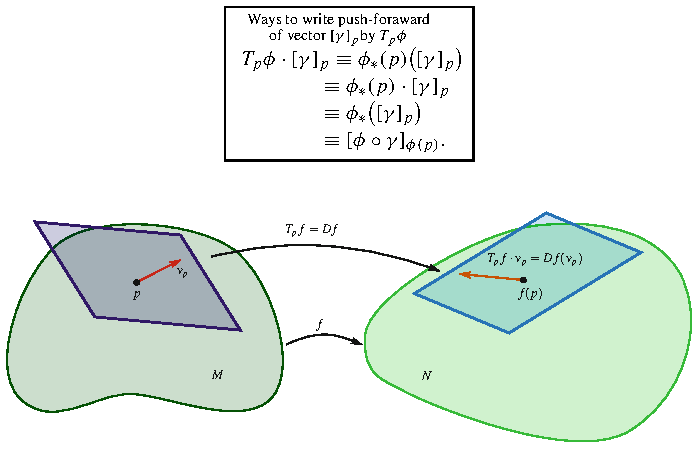
\includegraphics[width=0.830\linewidth]{images/vector/fig-10-17.pdf}
  \caption{给定流形之间的映射 $f:M\to N$，则 $f$ 诱导出前推映射 $Tf:TM\to TN$. 在特定点处，我们有 $T_pf:T_pM\to T_pN$}
  \label{fig:10-17}
\end{figure}

现在我们想从更抽象的角度来看这个. 假设我们有映射 $\phi:M\to N$，并且我们有一个由曲线 $\gamma$ 确定的向量 $v_p$. 我们想知道 $T_p\phi\cdot v_p$ 是什么. 从图~\ref{fig:10-18} 应该清楚，由映射 $\phi$ 对向量 $[\gamma]$ 的前推是曲线 $\phi\circ\gamma$. 于是我们把 $[\gamma]_p$ 被 $T_p\phi$ 的前推定义为
\begin{center}
\fbox{\parbox{0.92\textwidth}{\centering
向量 $[\gamma]_p$ 被 $T_p\phi$ 的前推：\\[0.4em]
$T_p\phi\cdot[\gamma]_p=[\phi\circ\gamma]_{\phi(p)}.$
}}
\end{center}

在很多方面，这是前推的一个更简洁的表述. 它也使抽象计算简单得多，我们将看到这一点. 在记法上，有几种不同的写法，它们都表示同一件事.

\begin{center}
\fbox{\parbox{0.92\textwidth}{\centering
写向量 $[\gamma]_p$ 被 $T_p\phi$ 前推的方式：\\[0.4em]
$T_p\phi\cdot[\gamma]_p\equiv\phi_*(p)\left([\gamma]_p\right)\equiv\phi_*(p)\cdot[\gamma]_p\equiv\phi_*\left([\gamma]_p\right)\equiv[\phi\circ\gamma]_{\phi(p)}.$
}}
\end{center}

\begin{figure}[htbp]
  \centering
  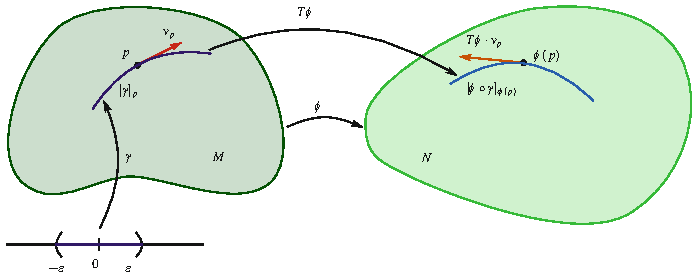
\includegraphics[width=0.960\linewidth]{images/vector/fig-10-18.pdf}
  \caption{这里我们有一个流形之间的映射 $\phi:M\to N$ 和一个向量 $[\gamma]_p\in T_pM$，其中 $\gamma:(-\epsilon,\epsilon)\to M$ 满足 $\gamma(0)=p$. 这个向量被 $T_p\phi$ 前推是什么？它就是由曲线 $\phi\circ\gamma$ 给出的向量，即 $[\phi\circ\gamma]_{\phi(p)}$}
  \label{fig:10-18}
\end{figure}

当然，所有这些记号也都可以省去基点来写：
\[
T\phi\cdot[\gamma]\equiv\phi_*([\gamma])\equiv\phi_*\cdot[\gamma]=[\phi\circ\gamma].
\]

回到我们熟悉的例子 $\phi:\mathbb{R}_{xy}^2\to\mathbb{R}_{uv}^2$，其中 $\phi(x,y)=\bigl(u(x,y),v(x,y)\bigr)=(x+y,x-y)$，我们可以看到计算一个向量的前推的这两种方式给出相同的答案. 再次考虑向量 $u_0=\binom{1}{2}\equiv[\gamma]_0$，其中
\[
\gamma:(-\epsilon,\epsilon)\longrightarrow\mathbb{R}_{xy}^2,\qquad t\longmapsto(t,2t).
\]

我们希望求 $u_0$ 被 $\phi$ 的前推. 首先我们通过求切映射 $T\phi$ 来做，然后利用它来求 $T\phi\cdot u_0$.
\[
T\phi=\phi_*=\begin{bmatrix}\dfrac{\partial u}{\partial x}&\dfrac{\partial u}{\partial y}\\[0.6em] \dfrac{\partial v}{\partial x}&\dfrac{\partial v}{\partial y}\end{bmatrix}=\begin{bmatrix}1&1\\1&-1\end{bmatrix}.
\]
我们不为这个矩阵担心基点，因为显然 $T\phi$ 不依赖于它所处的基点. 然后我们求 $u_0$ 的前推：
\[
T\phi\cdot u_0=\begin{bmatrix}1&1\\1&-1\end{bmatrix}\binom{1}{2}_{\phi(0)}=\binom{3}{-1}_0.
\]

现在我们用更抽象的向量曲线等价类定义来计算同样的东西：
\[
T\phi\cdot[\gamma]_0=[\phi\circ\gamma]_{\phi(0)}=[\phi\circ(t,2t)]_0=[(t+2t,t-2t)]_0=[(3t,-t)]_0.
\]

因此曲线 $\phi\circ\gamma=(3t,-t)$ 就是我们要找的前推向量. 也就是说，$T\phi\cdot u_0\equiv[(3t,-t)]_0$. 为了检验我们的答案是正确的，并且与上面得到的答案等价，我们必须对时间求这条曲线的导数：
\[
[\phi\circ\gamma]_{\phi(0)}'=\begin{bmatrix}\left.\dfrac{\partial(\phi\circ\gamma)_1(t)}{\partial t}\right|_{t=0}\\[1.2em] \left.\dfrac{\partial(\phi\circ\gamma)_2(t)}{\partial t}\right|_{t=0}\end{bmatrix}_{\phi(0)}=\begin{bmatrix}\left.\dfrac{\partial(3t)}{\partial t}\right|_{t=0}\\[1.2em] \left.\dfrac{\partial(-t)}{\partial t}\right|_{t=0}\end{bmatrix}_{\phi(0)}=\binom{3}{-1}_0,
\]
这正是我们想证明的.

\begin{question}\label{q:10-3}
对映射 $\phi:M\to N$ 和函数 $f:N\to\mathbb{R}$，证明 $v_p[f\circ\phi]=\left(T_p\phi\cdot v_p\right)_{\phi(p)}[f]$.
\end{question}

现在我们已经解决了向量的前推，我们想来看微分形式的拉回. 概念上，发生的事情并不难理解. 相关的映射定义为
\begin{align*}
\phi:M\longrightarrow N,\qquad p\longmapsto\phi(p) \\
T_p\phi:T_pM\longrightarrow T_{\phi(p)}N,\qquad v_p\longmapsto T_p\phi\cdot v_p,\qquad [\gamma]_p\longmapsto[\phi\circ\gamma]_{\phi(p)} \\
T_p^*M\longleftarrow T_{\phi(p)}^*N:T_p^*\phi,\qquad T_p^*\phi\cdot\alpha_{\phi(p)}\longleftarrow\alpha_{\phi(p)}
\end{align*}
并在图~\ref{fig:10-19} 中示出. 1-形式 $\alpha_{\phi(p)}\in T_{\phi(p)}^*N$ 的拉回是 $T_p^*\phi\cdot\alpha_{\phi(p)}\in T_p^*M$，它因此吃向量 $v_p\in T_pM$. 于是我们把 1-形式的拉回定义为
\[
\left(T_p^*\phi\cdot\alpha_{\phi(p)}\right)(v_p)\equiv\alpha_{\phi(p)}\left(T_p\phi\cdot v_p\right).
\]

\begin{figure}[htbp]
  \centering
  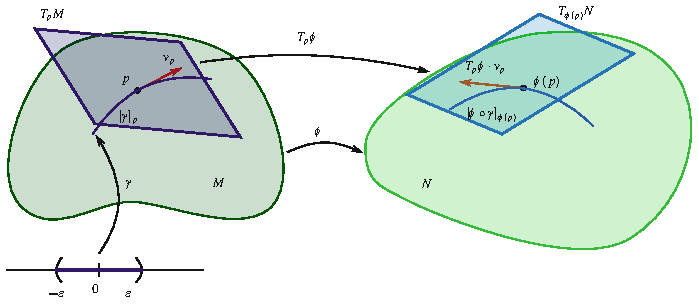
\includegraphics[width=0.960\linewidth]{images/vector/fig-10-19.pdf}
  \caption{这里说明了向量的前推与 1-形式的拉回之间的关系. 我们把余切空间 $T_p^*M$ 和 $T_{\phi(p)}^*N$ 画在切空间的上方，尽管切空间和余切空间都``附着''在流形的同一点上. 注意拉回映射与前推映射的方向相反}
  \label{fig:10-19}
\end{figure}

还要回想一下，给拉回映射标下标的是值域中的点 $p$，而不是定义域中的点. 这是一个相当不寻常的记法约定，但鉴于上面的定义，它使拉回与前推映射之间的联系显而易见. 利用我们在本节中引入的向量的曲线等价类定义，我们有拉回
\begin{center}
\fbox{\parbox{0.92\textwidth}{\centering
1-形式 $\alpha_{\phi(p)}$ 被 $T_p^*\phi$ 的拉回：\\[0.4em]
$\left(T_p^*\phi\cdot\alpha_{\phi(p)}\right)([\gamma]_p)\equiv\alpha_{\phi(p)}\left(T_p\phi\cdot[\gamma]_p\right)=\alpha_{\phi(p)}\left([\phi\circ\gamma]_{\phi(p)}\right).$
}}
\end{center}

这个等式用更传统的记号写起来实际上看起来非常简单. 这里我们省去基点来写拉回，这样你就能看到它实际上有多简单：
\begin{center}
\fbox{\parbox{0.92\textwidth}{\centering
$\phi^*\alpha([\gamma])=\alpha([\phi\circ\gamma]).$
}}
\end{center}

类似地，对于 $k$-形式 $\omega_{\phi(p)}\in\bigwedge_{\phi(p)}^k(N)$，我们得到拉回映射
\[
\bigwedge_p^k(M)\longleftarrow\bigwedge_{\phi(p)}^k(N):T_p^*\phi,\qquad T_p^*\phi\cdot\omega_{\phi(p)}\longleftarrow\omega_{\phi(p)},
\]
它定义为
\[
\left(T_p^*\phi\cdot\omega_{\phi(p)}\right)(v_{p_1},v_{p_2},\ldots,v_{p_k})\equiv\omega_{\phi(p)}\left(T_p\phi\cdot v_{p_1},T_p\phi\cdot v_{p_2},\ldots,T_p\phi\cdot v_{p_k}\right).
\]

用向量的曲线等价类定义，$k$-形式 $\omega$ 的拉回由下式给出，
\begin{center}
\fbox{\parbox{0.92\textwidth}{\centering
$k$-形式 $\omega_{\phi(p)}$ 被 $T_p^*\phi$ 的拉回：\\[0.4em]
$\left(T_p^*\phi\cdot\omega_{\phi(p)}\right)([\gamma_1]_p,[\gamma_2]_p,\ldots,[\gamma_k]_p)\equiv\omega_{\phi(p)}\left(T_p\phi\cdot[\gamma_1]_p,T_p\phi\cdot[\gamma_2]_p,\ldots,T_p\phi\cdot[\gamma_k]_p\right)$\\[0.4em]
$=\omega_{\phi(p)}\left([\phi\circ\gamma_1]_{\phi(p)},[\phi\circ\gamma_2]_{\phi(p)},\ldots,[\phi\circ\gamma_k]_{\phi(p)}\right).$
}}
\end{center}

我们还给出 0-形式的拉回的定义. 回想一下，流形 $N$ 上的 0-形式只是实值函数 $f:N\to\mathbb{R}$. 函数的拉回正是你所期望的，
\begin{center}
\fbox{\parbox{0.92\textwidth}{\centering
0-形式 $f$ 被 $T_p^*\phi$ 的拉回：\\[0.4em]
$T_p^*\phi\cdot f\equiv(f\circ\phi)(p)=f(\phi(p)).$
}}
\end{center}

这个定义用传统记法、且不含基点时看起来非常简单：
\begin{center}
\fbox{\parbox{0.92\textwidth}{\centering
0-形式 $f$ 被 $\phi^*$ 的拉回：\\[0.4em]
$\phi^*\cdot f\equiv f\circ\phi.$
}}
\end{center}

事实上，我们在第 6.7 节证明第三个恒等式 $\phi^*d=d\phi^*$ 时已经看到并使用过这一点.

\section{流形上的微积分}

没有理由不把你微积分和向量微积分课程中学到的所有微积分都归为``流形上的微积分''. 在这些情形中，流形只是欧几里得空间 $\mathbb{R}^2$ 或 $\mathbb{R}^3$. 然而，当人们听到流形上的微积分这个短语，或者流形上的积分、甚至流形上的分析等替代短语时，一般的假设是流形比欧几里得空间更复杂，是我们在本章引入的那种流形，即带有一个由坐标图 $(U_i,\phi_i)$ 组成的图册的那种流形.

\subsection{流形上的微分}

微积分一词当然既意味着微分也意味着积分. 本节我们将对流形上的微分做几点宏观的评论. 下一小节以及下一章将集中讨论流形上的积分. 人们经常遇到流形上的三种不同的微分概念. 这三种概念的作用方式都略有不同.

\begin{enumerate}
  \item \newterm{exterior-derivative}{外微分}{exterior derivative}：这是我们在本书中研究的那种微分，我们在第 4 章已经大量考察过外微分. 外微分作用于微分形式. 当微分形式是 0-形式，换言之只是一个函数时，外微分与微积分中的方向导数相同. 正如我们在第 4.5 节看到的，在很实在的意义上，外微分是我们的一般微积分课程中方向导数思想的推广. 也正是这种微分版本给出了将在第 11 章证明的推广 Stokes 定理. 这个推广的 Stokes 定理是流形上积分的重要组成部分. 最后，在第 4.3 节我们证明了外微分算子的局部存在性与唯一性. 现在我们已经有了必要的概念，下面将证明外微分算子的整体存在性与唯一性.
  \item Lie 导数：Lie 导数作用于称为\newterm{tensor}{张量}{tensor}的对象上. 微分形式实际上是张量的一个子集，所以谈论微分形式的 Lie 导数也完全说得通. 而且，Lie 微分有一个非常好的几何意义，比外微分更容易可视化和理解. 我们将在附录 A 中引入张量，并在第 A.7 节讨论 Lie 导数. 在那里我们导出几个把外微分与 Lie 微分联系起来的公式. 事实上，其中一个公式被用来通过归纳法证明整体外微分公式，该公式在第 4.4.2 节曾从某种几何的角度讨论过.
  \item \newterm{covariant-derivative}{协变导数}{covariant derivative}：本书完全不会讨论协变导数，但它们依赖于联络的概念，我们曾在第 10.1 节开头非常简略地讨论过. 如前所述，联络是流形上的附加结构，它``连接''切空间，以便告诉我们向量从一个切空间到另一个切空间的平行移动是什么. 其基本思想是，知道不同切空间中什么样的向量构成平行向量，使我们能够测量当张量和形式的输入向量被平行移动时它们如何变化. 协变导数是我们一般微积分课程中方向导数的第二种推广方式.
\end{enumerate}

你应该认识到，在讨论 $\mathbb{R}^2$ 或 $\mathbb{R}^3$ 时，这三种导数概念同样有效. 只是在你入门微积分课程中，你只对函数感兴趣，而不关心微分形式或张量. 除此之外，在我们流形中内置了一个非常自然且直观可理解的 $\mathbb{R}^2$ 或 $\mathbb{R}^3$ 上的欧几里得联络. 由于这些考虑，在一般微积分课程中实际上从来不需要讨论各种微分概念，老式的方向导数就足够了. 到你在向量微积分中时，你实际上确实学习了外微分，但正如你在第 9 章学到的，外微分被冠以梯度、旋度和散度这些专门的名称. 换言之，外微分的本质被不同的词汇和避免引入形式的企图掩盖了. 这就是为什么一切都保持为向量的原因.

但在更一般、更抽象的背景下，我们需要关注这些不同的微分概念. 有大量的恒等式把这些不同的导数思想彼此联系起来. 所有这些都使得流形上的微积分这个主题比欧几里得空间 $\mathbb{R}^2$ 或 $\mathbb{R}^3$ 上的微积分要复杂得多. 流形上的微积分实际上开始进入微分几何的领域，而上面提到的所有思想实际上将构成微分几何入门课程的主题.

说了这些之后，我们现在把注意力转向在微分形式的语境中很重要的一些基础内容. 我们首先简要地回到我们在第 4.3 节结束的地方. 在那节中，我们取了我们希望外微分具有的四个性质，称之为公理，然后导出了外微分的一般公式. 第四条公理基本上说明，在 0-形式的情形中，外微分必须与方向导数相同，从而确保外微分实际上是方向导数的推广. 然后我们利用这些公理导出了外导数的一般公式. 一旦我们做到了这一点，并有了一个一般微分形式的外导数的单一公式，我们就知道外微分算子 $d$ 必须既存在又唯一.

花点时间仔细回顾一下第 4.3 节. 注意两件事. 第一，第四条公理说明，在局部坐标下，对每个函数 $f$，都有 $df=\sum\frac{\partial f}{\partial x_i}dx_i$. 第二，我们曾假设我们有一个 n-形式
\[
\alpha=\sum\alpha_{i_1\cdots i_n}dx_{i_1}\wedge\cdots\wedge dx_{i_n}.
\]
在这两种情形中，我们都隐式地依赖一个坐标系，而且在该节的语境中，我们隐式地依赖笛卡尔坐标系. 但一般流形没有单一坐标系，相反它有一个由坐标片 $(U_i,\phi_i)$ 组成的图册 $\{(U_i,\phi_i)\}$. 第 4.3 节所做的一切只适用于单个坐标片 $(U_i,\phi_i)$. 当然，同样的论证和计算可以在许多坐标片中的每一个上进行，但这一切只意味着，在许多坐标片中的每一个上，我们都找到了一个给出微分形式外导数的公式，只要该形式用那个特定坐标片的坐标写出即可.

现在我们证明外微分算子 $d$ 整体存在且唯一. 这意味着 $d$ 在整个流形 $M=\bigcup U_i$ 上存在且唯一. 在坐标片 $(U_i,\phi_i)$ 上，我们证明了外微分算子存在且唯一，现在我们把它标为 $d_{U_i}$. 我们在这个坐标片上定义整体微分算子 $d$ 为 $d=d_{U_i}$. 类似地，在坐标片 $(U_j,\phi_j)$ 上，我们证明了外微分算子存在且唯一，现在我们把它标为 $d_{U_j}$. 我们同样在这个坐标片上定义整体微分算子 $d$ 为 $d=d_{U_j}$. 问题是，如果 $U_i\cap U_j\neq\emptyset$ 会怎样？由于 $d_{U_i}$ 在 $U_i$ 上存在且唯一，而 $d_{U_j}$ 在 $U_j$ 上存在且唯一，那么在 $U_i\cap U_j$ 上我们必须有 $d_{U_i}=d_{U_j}=d$. 由于这在所有坐标片的交上都成立，所以我们有 $d$ 整体存在且唯一，即在 $M=\bigcup U_i$ 上成立.

\subsection{流形上的积分}

现在我们把注意力转向流形上的积分. 既然流形上微分有好几种不同的思想，你就不应奇怪流形上积分也有不同的思想. 这里我们将把自己限制在讨论流形上微分形式的积分.

为了使一切都能顺顺利利地进行，我们将假设流形是可定向的. 当流形不可定向时也有办法做积分，但我们不在这里讨论它们.

\begin{definition}[可定向流形]\label{def:10-4-1}
可定向的 n 维流形 $M$ 是在流形的每一点处都有一个不为零的 n-形式的流形. 换言之，若 $fdx_1\wedge\cdots\wedge dx_n$ 是 $M$ 上的一个 n-形式，则不存在 $p\in M$ 使得 $f(p)=0$. 这意味着对所有点 $p\in M$，要么 $f(p)>0$，要么 $f(p)<0$. 具有这一性质的形式称为\newterm{nowhere-zero-n-form}{无处为零的 n-形式}{nowhere-zero n-form}. 于是，所有无处为零的 n-形式的集合分成两个等价类，一个等价类由所有处处为正的无处为零的 n-形式组成，第二个等价类由所有处处为负的无处为零的 n-形式组成. 通过选择这两个等价类中的一个，我们就规定了所谓的流形的\newterm{orientation}{定向}{orientation}.
\end{definition}

我们可以把定向想成允许我们以一致的方式求流形上的体积. 或者，我们可以把定向想成允许我们以一致的方式给所有切空间定向. 流形 $\mathbb{R}^n$ 的标准定向是包含无处为零的 n-形式 $dx_1\wedge\cdots\wedge dx_n$ 的那个等价类. 这个定向常常被描述为由 $dx_1\wedge\cdots\wedge dx_n$ 诱导的定向.

但注意我们在这里做了什么. 只要我们的流形有一个由单个坐标图组成的图册，说流形 $M$ 具有由 n-形式 $dx_1\wedge\cdots\wedge dx_n$ 诱导的定向就一切顺利. 但如果不是这样呢？考虑图~\ref{fig:10-20}，其中我们展示了一个带两个坐标图 $(U_i,\phi_i)$ 和 $(U_j,\phi_j)$（其中 $U_i\cap U_j\neq\emptyset$）的流形. $U_i$ 上的\newterm{volume-form}{体积形式}{volume form}会是什么样子？让我们考虑定义在整个 $\mathbb{R}^n$ 上的标准体积形式 $dx_1\wedge\cdots\wedge dx_n$，因此它显然定义在 $\phi_i(U_i)\subset\mathbb{R}^n$ 上. 我们可以把这个标准体积形式拉回到 $U_i\subset M$ 上. 因此，在某种意义上，$T^*\phi_i\cdot\left(dx_1\wedge\cdots\wedge dx_n\right)$ 是 $U_i\subset M$ 上的一个``标准''体积形式.

\begin{figure}[htbp]
  \centering
  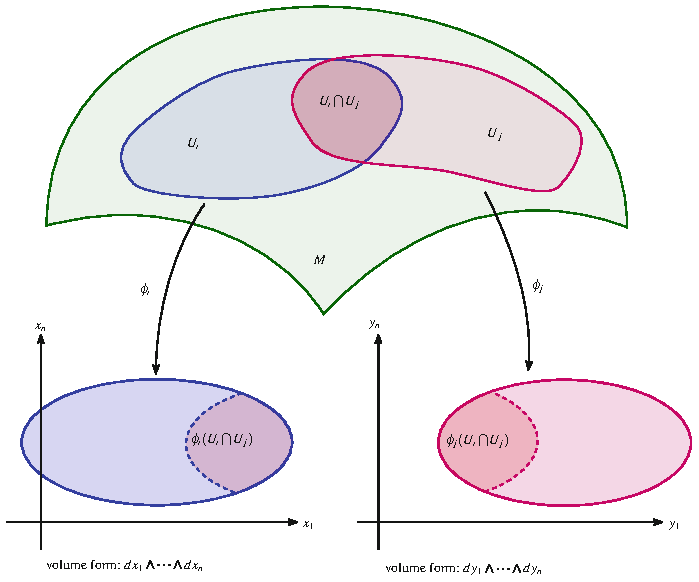
\includegraphics[width=0.952\linewidth]{images/vector/fig-10-20.pdf}
  \caption{带两个坐标图 $(U_i,\phi_i)$ 和 $(U_j,\phi_j)$（其中 $U_i\cap U_j\neq\emptyset$）的流形 $M$. $\mathbb{R}^n$ 的标准体积形式 $dx_1\wedge\cdots\wedge dx_n$ 在 $\phi_i(U_i)$ 和 $\phi_j(U_j)$ 上都存在}
  \label{fig:10-20}
\end{figure}

类似地，$U_j$ 上的体积形式会是什么样子？像以前一样，我们将考虑 $\phi_j(U_j)\subset\mathbb{R}^n$ 上的标准体积形式，为不把它与 $dx_1\wedge\cdots\wedge dx_n$ 混淆，我们称之为 $dy_1\wedge\cdots\wedge dy_n$. 我们可以把这个标准体积形式拉回到 $U_j\subset M$ 上，得到拉回 $T^*\phi_j\cdot\left(dy_1\wedge\cdots\wedge dy_n\right)$，作为 $U_j\subset M$ 上的一个``标准''体积形式. 这两个体积形式在它们都有定义的 $U_i\cap U_j$ 上如何相互关联？一般来说它们不会相同. 但要记住我们真正追求的是什么. 我们真正想要的是在整个 $M$ 上定义一个一致的体积形式 $\omega$，以便用它来定义 $M$ 上的定向.

在整个 $M$ 上寻找一个``一致的体积形式'' $\omega$ 实际上意味着什么？考虑图~\ref{fig:10-21}. 假设我们在 $\phi_j(U_j)$ 上有标准体积形式 $dy_1\wedge\cdots\wedge dy_n$. 如果 $\phi_i(U_i)$ 上存在一个体积形式 $f(x_1,\ldots,x_n)dx_1\wedge\cdots\wedge dx_n$，使得在 $U_i\cap U_j$ 上有
\[
T^*\phi_i\left(f(x_1,\ldots,x_n)dx_1\wedge\cdots\wedge dx_n\right)=T^*\phi_j\left(dy_1\wedge\cdots\wedge dy_n\right),
\]
那么我们就可以利用这两个体积形式（一个在 $U_j$ 上，一个在 $U_i$ 上）``缝合''出一个定义在 $U_i\cup U_j$ 上的体积形式. 通过反复这样做，我们可以``缝合''出一个定义在整个 $M$ 上的体积形式 $\omega$. 但首先我们需要在 $\phi_i(U_i)$ 上找到体积形式 $f(x_1,\ldots,x_n)dx_1\wedge\cdots\wedge dx_n$.

\begin{figure}[htbp]
  \centering
  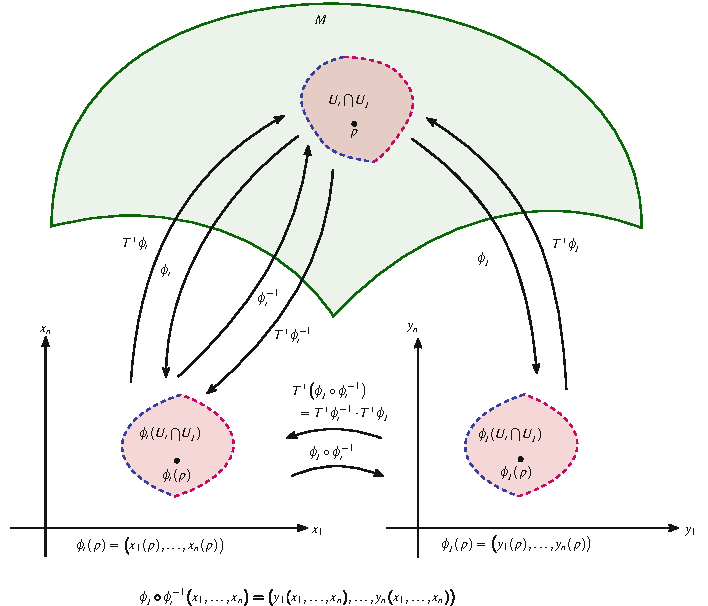
\includegraphics[width=0.949\linewidth]{images/vector/fig-10-21.pdf}
  \caption{这里我们聚焦于图~\ref{fig:10-20} 中的 $U_i\cap U_j$. 求 $T^*\left(\phi_j\circ\phi_i^{-1}\right)\left(dy_1\wedge\cdots\wedge dy_n\right)$ 所需的全部映射}
  \label{fig:10-21}
\end{figure}

看图~\ref{fig:10-21} 可以清楚看到，我们想要的等式
\[
T^*\phi_i\left(f(x_1,\ldots,x_n)dx_1\wedge\cdots\wedge dx_n\right)=T^*\phi_j\left(dy_1\wedge\cdots\wedge dy_n\right)
\]
等价于
\[
\begin{aligned}
f(x_1,\ldots,x_n)dx_1\wedge\cdots\wedge dx_n&=T^{*}\phi_i^{-1}\cdot T^*\phi_j\left(dy_1\wedge\cdots\wedge dy_n\right)\\
&=T^*\left(\phi_j\circ\phi_i^{-1}\right)\left(dy_1\wedge\cdots\wedge dy_n\right).
\end{aligned}
\]

我们实际上去求这个的方法是依靠映射
\[
\phi_j\circ\phi_i^{-1}(x_1,\ldots,x_n)=\left(y_1(x_1,\ldots,x_n),\ldots,y_n(x_1,\ldots,x_n)\right)
\]
把体积形式 $dy_1\wedge\cdots\wedge dy_n$ 写成用 $dx_1,\ldots,dx_n$ 表示的形式：
\[
\begin{aligned}
dy_1\wedge\cdots\wedge dy_n&=dy_1(x_1,\ldots,x_n)\wedge\cdots\wedge dy_n(x_1,\ldots,x_n)\\
&=\left(\frac{\partial y_1}{\partial x_1}dx_1+\cdots+\frac{\partial y_1}{\partial x_n}dx_n\right)\wedge\cdots\wedge\left(\frac{\partial y_n}{\partial x_1}dx_1+\cdots+\frac{\partial y_n}{\partial x_n}dx_n\right)\\
&=\underbrace{\begin{vmatrix}\dfrac{\partial y_1}{\partial x_1}&\cdots&\dfrac{\partial y_1}{\partial x_n}\\[1.2em] \vdots&\ddots&\vdots\\[0.6em] \dfrac{\partial y_n}{\partial x_1}&\cdots&\dfrac{\partial y_n}{\partial x_n}\end{vmatrix}}_{\text{$\phi_j\circ\phi_i^{-1}$ 的 Jacobian 行列式}}dx_1\wedge\cdots\wedge dx_n.
\end{aligned}
\]

于是，我们有
\[
T^*\left(\phi_j\circ\phi_i^{-1}\right)\left(dy_1\wedge\cdots\wedge dy_n\right)=\begin{vmatrix}\dfrac{\partial y_1}{\partial x_1}&\cdots&\dfrac{\partial y_1}{\partial x_n}\\[1.2em] \vdots&\ddots&\vdots\\[0.6em] \dfrac{\partial y_n}{\partial x_1}&\cdots&\dfrac{\partial y_n}{\partial x_n}\end{vmatrix}dx_1\wedge\cdots\wedge dx_n.
\]

一般地，$\phi_j\circ\phi_i^{-1}$ 的 Jacobian 矩阵的行列式可正可负，通常我们不会在意. 拉回 $dy_1\wedge\cdots\wedge dy_n$ 是什么就是什么. 然而，现在我们关心的是整个 $M$ 上一个一致的体积形式 $\omega$，这意味着在 $U_i\cap U_j$ 中，我们有
\[
T^*\phi_i\left(f(x_1,\ldots,x_n)dx_1\wedge\cdots\wedge dx_n\right)=T^*\phi_j\left(dy_1\wedge\cdots\wedge dy_n\right).
\]
由于 $dx_1\wedge\cdots\wedge dx_n$ 和 $dy_1\wedge\cdots\wedge dy_n$ 具有相同的定向，为了使上述等式的右边和左边具有相同的定向，我们需要 $\phi_j\circ\phi_i^{-1}$ 的 Jacobian 为正. 因此，只要映射 $\phi_i$ 和 $\phi_j$ 使得转移函数 $\phi_j\circ\phi_i^{-1}$ 有行列式为正的 Jacobian，我们就可以在 $U_i\cup U_j$ 上定义一个一致的体积形式.

把它推广到整个 $M$，只要 $M$ 有一个图册 $\{(U_i,\phi_i)\}$ 使得每个转移函数 $\phi_j\circ\phi_i^{-1}$ 都有行列式为正的 Jacobian，我们就可以在 $M$ 上找到一个一致的体积形式. 另一种说法是：只要流形 $M$ 容许一个转移函数有正 Jacobian 行列式的图册，它就是\newterm{orientable}{可定向的}{orientable}.

现在我们转向处理流形上积分所需的下一思想. 假设我们有一个带图册 $\{(U_i,\phi_i)\}$ 的流形 $M$. 由于 $\{(U_i,\phi_i)\}$ 是 $M$ 的一个图册，我们有 $M=\bigcup U_i$. 坐标片族 $\{U_i\}$ 称为 $M$ 的一个\newterm{covering}{覆盖}{covering}. 对每个坐标片 $U_i$，假设我们有一个只在 $U_i$ 的某个子集 $V$ 上非零的实值函数 $\varphi_i:M\to\mathbb{R}$. 换言之，若 $p\notin V\subset U_i$，则 $\varphi_i(p)=0$. 称函数 $\varphi_i$ 从属于坐标片 $U_i$.

\begin{definition}[单位分解]\label{def:10-4-2}
从属于覆盖 $\{U_i\}$ 的 $M$ 的\newterm{partition-of-unity}{单位分解}{partition of unity}是一族函数 $\varphi_i:M\to\mathbb{R}$，使得
\begin{enumerate}
  \item[(a)] 对 $M$ 的覆盖中的每个坐标片 $U_i$，我们有一个从属于坐标片 $U_i$ 的函数 $\varphi_i$，
  \item[(b)] 对所有 $p\in U_i$ 有 $0\leq\varphi_i(p)\leq 1$，并且
  \item[(c)] 对每个 $p\in M$ 有 $\sum_i\varphi_i(p)=1$.
\end{enumerate}
\end{definition}

如果流形 $M$ 可定向，通常假定用来构成 $M$ 的覆盖（即求单位分解时使用的覆盖）的图册，事实上就是转移函数有正 Jacobian 行列式的那个图册，也就是用来在 $M$ 上定义体积形式 $\omega$ 的那个图册.

单位分解使我们能够把任何微分形式 $\alpha$``分解''成一族从属于覆盖 $\{U_i\}$ 的微分形式，
\[
\alpha=\sum_i\varphi_i\alpha.
\]
显然 $\varphi_i\alpha$ 只在坐标片 $U_i$ 上非零. 我们实际上只能通过在覆盖多个坐标片的区域上把 $\alpha$ 分解成在每个坐标片上可积的形式来积分它. 因此例如，如果我们想在整个 $M$ 上积分 $\alpha$，我们将有
\[
\int_M\alpha=\int_M\sum_i\varphi_i\alpha=\sum_i\int_M\varphi_i\alpha=\sum_i\int_{U_i}\varphi_i\alpha,
\]
其中最后一个等号成立是因为 $M=\bigcup_iU_i$ 且 $\varphi_i\alpha$ 在 $U_i$ 之外为零. 如果我们在区域 $R\subset M$ 上积分，那么我们就有
\[
\int_R\alpha=\sum_i\int_{U_i\cap R}\varphi_i\alpha.
\]
所以，能在一个流形的任意区域上、甚至在整个 $M$ 上积分一个形式，归结为能在单个坐标片上积分. 现在我们把注意力转向在单个坐标片上积分一个形式 $\alpha$. 注意，我们改变记号，直接使用 $\alpha$ 而不是 $\varphi_i\alpha$.

我们首先假设 $\alpha$ 是 n 维流形 $M$ 上的 n-形式，并且我们想求 $\int_{U_i}\alpha$. 我们要做的全部事情就是把 $\alpha$ 拉回到 $\phi_i(U_i)$ 并在那里积分，换言之，
\[
\int_{U_i}\alpha=\int_{\phi_i(U_i)}T^*\phi_i^{-1}\cdot\alpha.
\]
如果让你积分实值函数 $f:M\to\mathbb{R}$，那么这实际上意味着我们要积分 n-形式 $f\omega$，其中 $\omega$ 是 $M$ 上的体积形式. 于是我们使用
\[
\int_{U_i}f\omega=\int_{\phi_i(U_i)}T^*\phi_i^{-1}\cdot(f\omega)=\int_{\phi_i(U_i)}f\circ\phi_i^{-1}\,T^*\phi_i^{-1}\cdot\omega.
\]

\begin{question}\label{q:10-4}
证明上式中第二个等号成立.
\end{question}

为了在 n 维流形 $M$ 上积分一个 $k$-形式 $\beta$（其中 $k<n$），我们需要一个 $k$ 维\newterm{submanifold}{子流形}{submanifold}来在其上积分. 不去深究子流形的技术定义，你可以把它本质上想成一个由映射 $\Phi:\mathbb{R}^k\to M$ 给出的参数化曲面 $\Sigma\subset M$. 这正是我们在第 7.4 节所做的，我们在那里在一维和二维参数化曲面上积分. 然后我们可以按如下方式在子流形 $\Sigma$ 上积分 $\beta$：
\[
\int_{\Sigma}\beta=\int_{\Phi^{-1}(\Sigma)}T^*\Phi\cdot\beta.
\]
所以，尽管本节的讨论相当抽象和理论化，事实证明我们已经为我们正在讨论的内容做了大量的具体例子.

这实际上只涵盖了流形上积分的非常基础的内容. 在第 11 章中，我们将通过证明一个关于流形上积分非常重要的定理来扩展这个主题，这个定理对大量数学都至关重要，称为推广的 Stokes 定理，或者通常简称为 Stokes 定理.

\section{小结、参考文献与问题}

\subsection{小结}

n 维流形是一个空间 $M$，它可被一族局部坐标邻域 $U_i$ 连同一一映射 $\phi_i:U_i\to\mathbb{R}^n$ 完全覆盖，这些映射称为坐标映射. $U_i$ 与 $\phi_i$ 合起来称为坐标片或坐标图，一般记为 $(U_i,\phi_i)$. 所有坐标图合在一起 $\{(U_i,\phi_i)\}$ 称为 $M$ 的坐标系或图册. 由于 $U_i$ 覆盖整个 $M$，我们写 $M=\bigcup U_i$. 又因 $\phi_i$ 是一一的，它可逆，所以 $\phi_i^{-1}$ 存在且良定义. 若两个坐标图有非空交集 $U_i\cap U_j\neq\emptyset$，则函数 $\phi_j\circ\phi_i^{-1}:\mathbb{R}^n\to\mathbb{R}^n$ 称为转移函数.

\[
\begin{array}{rcl}
U_i & : & \text{坐标邻域}\\
\phi_i:U_i\to\mathbb{R}^n & : & \text{坐标映射}\\
(U_i,\phi_i) & : & \text{坐标片/坐标图}\\
\left\{(U_i,\phi_i)\right\} & : & \text{坐标系/图册}\\
\phi_j\circ\phi_i^{-1}:\mathbb{R}^n\to\mathbb{R}^n & : & \text{转移函数}
\end{array}
\]

假设 $r\in U_i\cap U_j\neq\emptyset$，则 $\phi_i(r)\in\mathbb{R}^n$ 且 $\phi_j(r)\in\mathbb{R}^n$. 此外，$\phi_j\circ\phi_i^{-1}$ 把 $\phi_i(U_i\cap U_j)\subset\mathbb{R}^n$ 送到 $\phi_j(U_i\cap U_j)\subset\mathbb{R}^n$. 也就是说，$\phi_j\circ\phi_i^{-1}$ 是 $\mathbb{R}^n$ 的一个子集到 $\mathbb{R}^n$ 的另一个子集的映射，因此以 $\phi_i(U_i\cap U_j)$ 为定义域、以 $\phi_j(U_i\cap U_j)$ 为值域的映射 $\phi_j\circ\phi_i^{-1}:\mathbb{R}^n\to\mathbb{R}^n$，是我们知道如何从多元微积分求导的那种映射. 微分流形是一个集合 $M$，连同坐标图族 $(U_i,\phi_i)$，其中 $M=\bigcup U_i$，使得每个映射 $\phi_j\circ\phi_i^{-1}$（其中 $U_i\cap U_j\neq\emptyset$）都是可微的.

我们用 $M$ 上的曲线定义 $M$ 在点 $p$ 处的切空间 $T_pM$. 若两条曲线在靠近 $p$ 处有相同的值域，且在靠近 $p$ 处有相同的参数化，则称它们等价，记为 $\sim$. 所有等价曲线的集合称为等价类，定义为
\[
[\gamma_1]\equiv\left\{\gamma\mid\gamma\sim\gamma_1\right\}.
\]
点 $p$ 处曲线的每个等价类被定义为 $p$ 处的一个切向量. $M$ 在 $p$ 处的切空间被定义为点 $p$ 处所有切向量（即曲线的等价类）的集合，
\[
T_pM=\left\{[\gamma]_p\mid\gamma:(-\epsilon,\epsilon)\to M\text{ 且 }\gamma(0)=p\right\}.
\]

切空间的等价类（内蕴）定义与向量（外蕴）定义之间的关系总结如下，
\[
\begin{array}{c|c|c}
\hline
\text{等价类定义} & \Longleftrightarrow & \underline{\text{向量定义}}\\
\hline
v_p=[\gamma]_p,\quad p=\gamma(0) & & v_p=[\gamma']_p=[\gamma]_p'\\
=\left[\left(\gamma_1(t),\ldots,\gamma_n(t)\right)\right] & & =\left[\left(\gamma_1'(t),\ldots,\gamma_n'(t)\right)\right]_p\\
& & =\left[\left(\gamma_1(t),\ldots,\gamma_n(t)\right)\right]_p'\\
& & =\begin{bmatrix}\gamma_1'(t=0)\\ \vdots\\ \gamma_n'(t=0)\end{bmatrix}_p\\
& & =\begin{bmatrix}\left.\dfrac{\partial\gamma_1(t)}{\partial t}\right|_{t=0}\\[1.2em] \vdots\\[0.6em] \left.\dfrac{\partial\gamma_n(t)}{\partial t}\right|_{t=0}\end{bmatrix}_p\\
\hline
\end{array}
\]

曲线的等价类定义给了我们思考链式法则的另一种方式，
\begin{center}
\fbox{\parbox{0.92\textwidth}{\centering
曲线情形的链式法则：\\[0.4em]
$[f\circ\phi^{-1}\circ\phi\circ\gamma]_0'=[f\circ\phi^{-1}]_{\phi\circ\gamma(0)}'\cdot[\phi\circ\gamma]_0'=[f\circ\phi^{-1}]_{\phi(p)}'\cdot[\phi\circ\gamma]_0'.$
}}
\end{center}

对于向量的等价类定义，$[\gamma]_p$ 被 $T_p\phi$ 的前推是
\begin{center}
\fbox{\parbox{0.92\textwidth}{\centering
$T_p\phi\cdot[\gamma]_p=[\phi\circ\gamma]_{\phi(p)}.$
}}
\end{center}

记法上有几种不同的写法，都表示同一件事：
\begin{center}
\fbox{\parbox{0.92\textwidth}{\centering
$T_p\phi\cdot[\gamma]_p\equiv\phi_*(p)\left([\gamma]_p\right)\equiv\phi_*(p)\cdot[\gamma]_p\equiv\phi_*\left([\gamma]_p\right)\equiv[\phi\circ\gamma]_{\phi(p)}.$
}}
\end{center}

在向量的曲线等价类定义中，$k$-形式 $\omega$ 的拉回由下式给出，
\begin{center}
\fbox{\parbox{0.92\textwidth}{\centering
$\left(T_p^*\phi\cdot\omega_{\phi(p)}\right)([\gamma_1]_p,[\gamma_2]_p,\ldots,[\gamma_k]_p)\equiv\omega_{\phi(p)}\left(T_p\phi\cdot[\gamma_1]_p,T_p\phi\cdot[\gamma_2]_p,\ldots,T_p\phi\cdot[\gamma_k]_p\right)$\\[0.4em]
$=\omega_{\phi(p)}\left([\phi\circ\gamma_1]_{\phi(p)},[\phi\circ\gamma_2]_{\phi(p)},\ldots,[\phi\circ\gamma_k]_{\phi(p)}\right),$
}}
\end{center}
而 0-形式（函数）$f:N\to\mathbb{R}$ 的拉回是
\begin{center}
\fbox{\parbox{0.92\textwidth}{\centering
$T_p^*\phi\cdot f\equiv(f\circ\phi)(p)=f(\phi(p)).$
}}
\end{center}
这个定义用传统记法且不含基点时看起来非常简单：
\begin{center}
\fbox{\parbox{0.92\textwidth}{\centering
$\phi^*\cdot f\equiv f\circ\phi.$
}}
\end{center}

虽然这远不是对流形的完整导引，但我们尝试提供了与一般流形 $M$ 相关的基本思想. 特别是，坐标图和图册的思想是定义一般流形的核心要素. 我们还试图说明，尤其是在第 10.4 节中，对坐标图保持谨慎有多么重要，以及它确实给流形上的微积分研究增加了额外一层的复杂性. 处理它通常并不困难，但确实需要注意这额外的一层复杂性. 由于这主要是一本关于微分形式的书，我们在本书的大部分内容中都试图避免这额外的一层复杂性，坚持使用欧几里得流形 $\mathbb{R}^n$，它们都有一个由一个坐标图构成的图册，即我们非常熟悉的欧几里得坐标图.

\subsection{参考文献与进一步阅读}

关于流形理论的书籍有数百本，这里介绍的一切都是相当标准的. 如果要说有什么的话，那就是鉴于对流形的这一导引如此简短，我们牺牲了数学严格性以换取可读性和可理解性. 本章旨在仅仅是对某些基础的非常基本的导引，足以让读者开始阅读更高级的书. 下面五本参考文献都很好，按难度递增的顺序给出：Munkres~\cite{ref35}、Walschap~\cite{ref47}、Renteln~\cite{ref37}、Martin~\cite{ref33} 和 Conlon~\cite{ref10}. 此外，Bishop 与 Crittenden~\cite{ref05} 以及 do Carmo~\cite{ref14} 这两本年代稍久一些的书也很不错，如果你能找到它们的话.

\subsection{问题}

\begin{question}\label{q:10-5}
把流形 $\mathbb{R}^2$ 上的下列向量写成三种不同形式的曲线等价类. （考虑使用三角函数或指数函数可能会有所帮助.）
\begin{enumerate}
  \item[(a)] $\binom{2}{3}_{(2,1)}$
  \item[(b)] $\binom{-4}{5}_{(3,-2)}$
  \item[(c)] $\binom{7}{-3}_{(-3,-1)}$
  \item[(d)] $\binom{-3}{-7}_{(-4,8)}$
  \item[(e)] $\binom{3}{1}_{(3,-2)}$
\end{enumerate}
\end{question}

\begin{question}\label{q:10-6}
利用问题~\ref{q:10-5} 中写成曲线等价类的向量 $v_p$，对下列函数 $f_i$ 求 $v_p[f_i]$. 验证无论你使用曲线的三种表示中的哪一种，都得到相同的答案.
\begin{enumerate}
  \item[(a)] $f_1(x,y)=xy^2$
  \item[(b)] $f_2(x,y)=y+\cos(x)$
  \item[(c)] $f_3(x,y)=e^x+3y-4$
  \item[(d)] $f_4(x,y)=\sqrt{xy}+xy$
  \item[(e)] $f_5(x,y)=(x+2y)^2$
\end{enumerate}
\end{question}

\begin{question}\label{q:10-7}
把流形 $\mathbb{R}^3$ 上的下列向量写成三种不同形式的曲线等价类. （考虑使用三角函数或指数函数可能会有所帮助.）
\begin{enumerate}
  \item[(a)] $\begin{bmatrix}4\\-2\\-8\end{bmatrix}_{(5,-2,4)}$
  \item[(b)] $\begin{bmatrix}3\\-6\\5\end{bmatrix}_{(3,-4,5)}$
  \item[(c)] $\begin{bmatrix}-4\\7\\-1\end{bmatrix}_{(2,4,-3)}$
  \item[(d)] $\begin{bmatrix}5\\9\\-9\end{bmatrix}_{(6,-4,2)}$
  \item[(e)] $\begin{bmatrix}-5\\-2\\-3\end{bmatrix}_{(7,3,-4)}$
\end{enumerate}
\end{question}

\begin{question}\label{q:10-8}
利用问题~\ref{q:10-7} 中写成曲线等价类的向量 $v_p$，对下列函数 $f_i$ 求 $v_p[f_i]$. 验证无论你使用曲线的三种表示中的哪一种，都得到相同的答案.
\begin{enumerate}
  \item[(a)] $f_1(x,y,z)=xy^2z$
  \item[(b)] $f_2(x,y,z)=y+\cos(x)+\sin(z)$
  \item[(c)] $f_3(x,y,z)=e^x+ye^z$
  \item[(d)] $f_4(x,y,z)=\sqrt{xyz}+xyz$
  \item[(e)] $f_5(x,y,z)=(x+2y-3z)^2$
\end{enumerate}
\end{question}

\begin{question}\label{q:10-9}
设 $\phi:\mathbb{R}^2\to\mathbb{R}^2$ 由 $\phi(x,y)=(2y,3x)$ 给出. 利用问题~\ref{q:10-5} 中向量 $v_p$ 的曲线等价类版本求 $T\phi\cdot v_p$. 验证你的答案不依赖于你使用的代表曲线.
\end{question}

\begin{question}\label{q:10-10}
设 $\phi:\mathbb{R}^2\to\mathbb{R}^2$ 由 $\phi(x,y)=(3x+2y,3x-2y)$ 给出. 利用问题~\ref{q:10-5} 中向量 $v_p$ 的曲线等价类版本求 $T\phi\cdot v_p$. 验证你的答案不依赖于你使用的代表曲线.
\end{question}

\begin{question}\label{q:10-11}
设 $\phi:\mathbb{R}^2\to\mathbb{R}^2$ 由 $\phi(x,y)=(xy,xy^3)$ 给出. 利用问题~\ref{q:10-5} 中向量 $v_p$ 的曲线等价类版本求 $T\phi\cdot v_p$. 验证你的答案不依赖于你使用的代表曲线.
\end{question}

\begin{question}\label{q:10-12}
设 $\phi:\mathbb{R}^3\to\mathbb{R}^3$ 由 $\phi(x,y,z)=(-2z,3x,-4y)$ 给出. 利用问题~\ref{q:10-7} 中向量 $v_p$ 的曲线等价类版本求 $T\phi\cdot v_p$. 验证你的答案不依赖于你使用的代表曲线.
\end{question}

\begin{question}\label{q:10-13}
设 $\phi:\mathbb{R}^3\to\mathbb{R}^3$ 由 $\phi(x,y,z)=(3x+2y+z,3x-2y+z,5z+7)$ 给出. 利用问题~\ref{q:10-7} 中向量 $v_p$ 的曲线等价类版本求 $T\phi\cdot v_p$. 验证你的答案不依赖于你使用的代表曲线.
\end{question}

\begin{question}\label{q:10-14}
设 $\phi:\mathbb{R}^3\to\mathbb{R}^3$ 由 $\phi(x,y,z)=(xy,yz,zx)$ 给出. 利用问题~\ref{q:10-7} 中向量 $v_p$ 的曲线等价类版本求 $T\phi\cdot v_p$. 验证你的答案不依赖于你使用的代表曲线.
\end{question}

\begin{question}\label{q:10-15}
设 $\phi:\mathbb{R}^2\to\mathbb{R}^2$ 由 $\phi(x,y)=\bigl(u(x,y),v(x,y)\bigr)=(2y,3x)$ 给出，并设 $\alpha=3v\,du+2u\,dv$. 在问题~\ref{q:10-5} 的每个向量处求 $T^*\phi\cdot\alpha$. 验证你的答案不依赖于你使用的代表曲线.
\end{question}

\begin{question}\label{q:10-16}
设 $\phi:\mathbb{R}^2\to\mathbb{R}^2$ 由 $\phi(x,y)=\bigl(u(x,y),v(x,y)\bigr)=(3x+2y,3x-2y)$ 给出，并设 $\alpha=\cos(u)\,du+\sin(v)\,dv$. 在问题~\ref{q:10-5} 的每个向量处求 $T^*\phi\cdot\alpha$. 验证你的答案不依赖于你使用的代表曲线.
\end{question}

\begin{question}\label{q:10-17}
设 $\phi:\mathbb{R}^2\to\mathbb{R}^2$ 由 $\phi(x,y)=\bigl(u(x,y),v(x,y)\bigr)=(xy,xy^3)$ 给出，并设 $\alpha=(2u+v)\,du+u^2v^3\,dv$. 在问题~\ref{q:10-5} 的每个向量处求 $T^*\phi\cdot\alpha$. 验证你的答案不依赖于你使用的代表曲线.
\end{question}

\begin{question}\label{q:10-18}
设 $\phi:\mathbb{R}^3\to\mathbb{R}^3$ 由
\[
\phi(x,y,z)=\bigl(u(x,y,z),v(x,y,z),w(x,y,z)\bigr)=(-2z,3x,-4y)
\]
给出，并设 $\alpha=2w\,du+3v\,dv+4u\,dw$. 在问题~\ref{q:10-7} 的每个向量处求 $T^*\phi\cdot\alpha$. 验证你的答案不依赖于你使用的代表曲线.
\end{question}

\begin{question}\label{q:10-19}
设 $\phi:\mathbb{R}^3\to\mathbb{R}^3$ 由 $\phi(x,y,z)=\bigl(u(x,y,z),v(x,y,z),w(x,y,z)\bigr)=(3x+2y+z,3x-2y+z,5z+7)$ 给出，并设 $\alpha=\sin(v)\,du+\cos(u)\,dv+3w\,dw$. 在问题~\ref{q:10-7} 的每个向量处求 $T^*\phi\cdot\alpha$. 验证你的答案不依赖于你使用的代表曲线.
\end{question}

\begin{question}\label{q:10-20}
设 $\phi:\mathbb{R}^3\to\mathbb{R}^3$ 由 $\phi(x,y,z)=\bigl(u(x,y,z),v(x,y,z),w(x,y,z)\bigr)=(xy,yz,zx)$ 给出，并设 $\alpha=(u+v)\,du+(v+w)\,dv+(w+u)\,dw$. 在问题~\ref{q:10-7} 的每个向量处求 $T^*\phi\cdot\alpha$. 验证你的答案不依赖于你使用的代表曲线.
\end{question}
